\RequirePackage{setspace}
\documentclass[nostrict]{pg_class}

\usepackage{listing_style}

\usepackage{csquotes}
\usepackage[polish, USenglish]{babel}
\usepackage{url}
\usepackage{enumitem}
\usepackage{float}
\usepackage{amsmath}
\usepackage{mathspec}
\usepackage{afterpage}
\usepackage{array}
\usepackage{booktabs}
\usepackage{multirow}
\usepackage{hyperref}
\usepackage{tikz}
\usepackage[bottom]{footmisc}
\usepackage[mode=buildmissing]{standalone}

%\RequirePackage{fontspec}
%\setmainfont{Arial}

\begin{document}
\selectlanguage{polish}
\def\UrlBreaks{\do\/\do-}
\setlist[enumerate]{labelsep=5pt, listparindent=0.9cm, itemsep=2pt} 
\setlist[itemize]{labelsep=5pt, listparindent=0.9cm, itemsep=2pt} 
\newcommand\img[5][]{
	\begin{figure}[H]
		\begin{center}
			\includegraphics[width=#5\textwidth]{#2}
			\bigskip
			\caption[#3]{#3 #1}
			\label{fig:#4}
		\end{center}
	\end{figure}
} 

\newcommand\drow[1]{\multirow{2}{*}{#1}}
\newcolumntype{x}[1]{>{\centering\arraybackslash\hspace{0pt}}m{#1}}
\newcommand\centertable[4]{
	\bigskip
	\begin{table}[H]
		\caption{#3}
		\label{tab:#4}
		\begin{center}
			\bgroup
			\def\arraystretch{1}
			\begin{tabular}{ #2 }
				#1
			\end{tabular}
			\egroup
		\end{center}
	\end{table}
}

\newcommand\codeinline[1]{\lstinline[basicstyle=\normalsize\ttfamily]{#1}}

\makeatletter
\newcommand{\sectionauthor}[1]{
{\vspace*{-5pt}\hspace*{4pt}\footnotesize\itshape\MakeUppercase{#1}
\par\nobreak\vspace*{10pt}}
\@afterheading}
\makeatother

\newcommand\blankpage{%
    \null
    \thispagestyle{empty}%
    \addtocounter{page}{-1}%
    \newpage}

\newcounter{appendices}
\setcounter{appendices}{0}

\newcommand\annex[2]{
	\cleardoublepage
	\phantomsection
	\refstepcounter{appendices}
	\addcontentsline{toc}{chapter}{Załącznik nr \theappendices: #1}
	\section*{Załącznik nr \theappendices: #1}
	\label{anx:#2}
}

\newcommand\annexref[2][]{\hyperref[anx:#2]{Załącznik#1~nr~\ref{anx:#2}}}

\newcommand\ang[1]{(ang.\textit{ #1})}

%\lstset{style=java}

%\includepdf[pages=-]{meta/title_page.pdf}
%\includepdf{meta/statement.pdf}
%\afterpage{\blankpage}

%\setcounter{page}{5}
\chapter*{Streszczenie}
Wraz~ze~stale postępującym wzrostem użycia komputerów, programów, serwisów internetowych~i~aplikacji mobilnych zwiększa się zapotrzebowanie~na~narzędzia~i~rozwiązania pomagające monitorować ich działanie oraz analizować zachowanie użytkowników~w~celu lepszego spełniania ich celów~i~poprawy jakości używanych~przez~nich produktów. Jednocześnie ostatnie postępy technologiczne, stały wzrost dostępnej mocy obliczeniowej oraz postępująca miniaturyzacja komponentów elektronicznych umożliwiły powstanie nowej kategorii rozwiązań, które interpretują sygnały dostępnych~w~urządzeniach sensorów. 

Niniejsza praca stanowi podsumowanie aktualnego stanu rozwoju aplikacji~i~platform monitorujących urządzenia~i~zachowania użytkowników. Omówione~i~porównane zostały przykłady rozwiązań pochodzących zarówno~z~środowiska akademickiego, jak~i~sektora komercyjnego. Ich różnorodność jest widoczna zarówno~na~poziomie ich budowy, działania oraz zastosowania. Przeprowadzony przegląd literatury naukowej ocenia postępy~w~pracach badawczych~nad~wykorzystaniem czujników~do~wykrywania aktywności ludzkich. Z~wyjątkiem paru publikacji zajmujących się oryginalnymi tematami większość~z~przeanalizowanych prac naukowych stanowi próbę ponownego podejścia~do~problemu wykrywania tego samego zestawu podstawowych aktywności~ze~zwiększoną dokładnością. 

Druga część pracy skupia się~na~zagadnieniu tworzenia map cieplnych~z~interakcji użytkowników~z~interfejsami aplikacji mobilnych. Szczegółowo opisany został proces tworzenia oryginalnego rozwiązania tego typu, rozpoczynając~od~projektu~i~architektury, przechodząc~przez~implementację~i~napotkane~w~jej trakcie wyzwania, kończąc~na~testach~i~publikacji. Końcowa część pracy poświęcona jest ewaluacji stworzonego rozwiązania,~w~ramach której odpowiednio przygotowana aplikacja została rozprowadzona~w~grupie testujących~ją~użytkowników. Zebrane dane~o~ich działaniach,~po~przetworzeniu~na~mapy cieplne, posłużyły~do~identyfikacji problemów~z~obsługą interfejsu aplikacji, identyfikacji dobrych praktyk jego projektowania oraz lepszego zrozumienia innych potencjalnych zastosowań tego typu rozwiązania. Wykorzystanie map cieplnych~do~wizualizacji interakcji daje unikalny wgląd~w~aplikację widzianą oczami użytkowników~i~pozwala~na~wyciągnięcie ważnych wniosków dotyczących jej interfejsu. \\

\noindent\textbf{Słowa kluczowe:} monitorowanie, aktywności, analiza, użytkownicy, zachowania, czujniki, aplikacje, mapy cieplne, interakcje, wizualizacja, interfejs, dostępność, przetwarzanie, ewaluacja \\

\noindent\textbf{Dziedzina nauki~i~techniki, zgodnie~z~wymogami OECD:} Nauki inżynierskie~i~techniczne, Elektrotechnika, elektronika, inżynieria informatyczna, Sprzęt komputerowy~i~architektura komputerów

\chapter*{Abstract}
Steadily increasing use of computers, programs, websites and mobile applications creates~a~demand for tools and solutions that monitor their operation and analyze user behavior. Those tools support developers in improving the quality of their products and help customers achieve their goals. At the same time, the price of electronic components such~as~sensors is rapidly falling, while the available computing power is increasing. Those factors have enabled the creation of~a~new category of products that interpret and use the signals emitted~by~sensors.

This paper summarizes the current state of development of~a~wide range of monitoring solutions created~by~both academia and commercial sectors. It includes examples of frameworks, device and user behavior monitoring tools and mobile sensor applications. Both their form and intended use varies considerably, even in the limited scope of chosen examples. Systematic literature review of scientific publications was conducted~to~assess the progress in research~on~the use of sensors~to~detect human activities. Except for~a~handful of original publications, most of the analyzed research papers approach~a~common problem of detecting the same set of basic activities attempting~to~achieve an increase in accuracy.

The second part of this document focuses~on~the issue of creating heat maps from user interactions with mobile applications. The process of creating an original solution for that purpose is described in detail, starting with the design and architecture, going through the implementation and encountered challenges and finishing with tests and release. The final part of this paper describes its evaluation process. A~mobile application outfitted with the created tool was distributed~to~the group of testers. Collected data was processed into heat maps which were then used~to~identify issues with the application user interface, come up with good design practices and better understand other potential uses of such tool. Conclusions that were based~on~the insight gained into the application usage validate the usefulness of using heat maps~to~visualize user interactions. \\

\noindent\textbf{Keywords:} monitoring, activities, analysis, users, behavior, sensors, applications, heat maps, interactions, visualization, interface, accessibility, processing, evaluation


\tableofcontents

\chapter*{Wykaz ważniejszych oznaczeń i skrótów}

\begin{description}
	\item [Systematyczny Przegląd Literatury] 
\end{description}



\begin{chapter}{Wstęp}
	\newcommand{\chapterPath}{chapters/Introduction}
% problemy zagadnienia
% badania metody

	\section{Kontekst pracy}
	Praca poświęcona jest tematowi rozwiązań informatycznych, których celem jest monitorowanie, zbieranie oraz przetwarzanie informacji~o~aplikacjach mobilnych, oraz działaniach, aktywności oraz zachowaniu ich użytkowników. Rozwój tej dziedziny jest spowodowany stale zwiększającym się rynkiem potencjalnych użytkowników oprogramowania~i~wiążącą się~z~nim rosnącą wartością tego typu danych. Wiedza użyciu produktu~i~występujących problemach jest podstawą przy podejmowaniu wielu decyzji biznesowych. Jeśli zostanie dobrze zastosowana, może mieć duży wpływ~na~jakość, popularność produktu oraz związane~w~nim wyniki finansowe. Jednocześnie postępujący spadek cen wielu komponentów elektronicznych, takich jak czujniki,~a~także stale zwiększająca się moc obliczeniowa, która jest głównym ogranicznikiem  przy przetwarzaniu zebranych~z~nich informacji umożliwia rozwój nowej kategorii inteligentnych rozwiązań monitorujących swoje otoczenie. Czynnikiem mającym szczególny wpływ~na~wiele nowych, innowacyjnych rozwiązań~w~tej kategorii jest rozwój~w~dziedzinie uczenia maszynowego~i~sztucznych sieci neuronowych, które dobrze nadają się~do~tego typu zastosowań.
	
	\section{Cele pracy}
	Głównym celem pracy jest przeanalizowanie~i~porównanie różnych mechanizmów monitorowania aktywności użytkowników aplikacji mobilnych oraz implementacja wybranego mechanizmu~w~aplikacji terapeutycznej. Analiza rozwiązań~i~osiągnięć, zarówno~w~sektorze otwartego oprogramowania, komercyjnym jak~i~akademickim,~ma~na celu stworzenie możliwie szerokiego przeglądu stanu aktualnie istniejącego oprogramowania monitorującego aktywności użytkowników. Celem tworzonego narzędzia jest ułatwienie~i~automatyzacja procesu zbierania~i~analizy danych~o~interakcjach użytkowników~z~interfejsami aplikacji mobilnych. Jednocześnie zastosowanie odpowiedniego sposobu wizualizacji zebranych danych~ma~zwiększyć ich przydatność mierzoną~w~ilości uzyskanych~z~analizy wniosków. Dodatkowym zamierzeniem projektu jest innowacja~w~obszarze oferowanych funkcji~i~możliwości wyróżniających stworzone narzędzie~na~tle innych rozwiązań tej samej kategorii.
	
	\section{Organizacja dokumentu}
	Na początku przedstawione~i~opisane zostały przykłady istniejących rozwiązań monitorujących, aplikacji przetwarzających dane~z~czujników, obserwujących użycie urządzeń,~na~których działają oraz platform mających~za~zadanie monitorowanie aplikacji~i~ich użytkowników. Kolejny rozdział zawiera sprawozdanie~z~przeprowadzonego~w~ramach pracy systematycznego przeglądu literatury naukowej dotyczącej tematu wykorzystania danych~z~sensorów~do~przewidywania zachowań~i~aktywności. Pytanie bazowe,~na~którego podstawie formułowane było zapytanie, brzmiało: {\it ``Jakie metryki~są~używane~do~opisu ludzkiej aktywności?''}. 
	
	Dalsza część pracy skupia się~na~wybranym zagadnieniu~z~obszaru monitorowania, czyli wizualizacji interakcji użytkowników~z~urządzeniami~w~postaci map cieplnych. Po~przedstawieniu tej techniki~i~jej najczęstszych zastosowań wymienione zostały przykłady istniejących produktów oferujących usługi~z~zakresu zbierania~i~prezentacji interakcji~w~formie map cieplnych. Następnie szczegółowo opisany jest proces projektowania, tworzenia~i~publikacji oryginalnego narzędzia tego typu. Przedstawione zostały też aspekty testów, dokumentacji~i~innych użytych~w~celu zapewnienia jakości rozwiązań. Napotkane~w~czasie implementacji wyzwania~są~zawarte~w~kolejnym rozdziale,~po~którym następuje szczegółowy opis procesu ewaluacji stworzonego narzędzia, rozpoczynający się~od~przygotowania~i~weryfikacji~a~kończący~na~walidacji~i~wnioskach końcowych. Wymieniona jest także lista pomysłów~i~usprawnień, które stanowią dobry punkt wyjścia przy dalszej pracy~nad~projektem.
\end{chapter}

\begin{chapter}{Przegląd istniejących rozwiązań monitorujących}
	\label{cha:existing_solutions}
	\newcommand{\chapterPath}{chapters/Existing_solutions}

	Wykrywanie aktywności~i~zachowań ludzkich~z~pomocą technologii jest zagadnieniem szerokim~i~wielowarstwowym. W celu pogłębienia swojej wiedzy, zapoznania się~z~osiągnięciami naukowymi~w~tej dziedzinie oraz zebrania materiałów~do~pracy został przeprowadzony \textit{Systematyczny Przegląd Literatury}. Bazował~on~na~publikacjach naukowych zebranych~z~pomocą trzech wyszukiwarek: \textit{Web of Science}, \textit{IEEE Explore} oraz \textit{PubMed}. 

Trzystopniowa selekcja pozwoliła~na~wyizolowanie najciekawszych~i~najlepiej pasujących~do~postawionego pytania artykułów. Wybrane publikacje zostały, zależnie~od~ich oceny, przeczytane~lub~przejrzane. Jednocześnie tworzone były interesujące~z~punktu widzenia tego przeglądu statystyki. 

Dużym zaskoczeniem~po~zapoznaniu się zebranymi materiałami był fakt~że~pomimo dużej powierzchownej  różnorodności większość~z~opisywanych eksperymentów skupiało się~na~wykrywaniu tego samego,~lub~bardzo podobnego zbioru modalności zawierającego zwykle chodzenie, siedzenie, stanie oraz leżenie. Ze względu~na~ich charakterystykę najodpowiedniejszy~do~ich wykrywania jest akcelerometr, który~z~tego powodu okazał się najczęściej wykorzystywanym sensorem.

Mimo~to~dzięki przeprowadzeniu przeglądu udało się zidentyfikować parę oryginalnych publikacji które przyczyniły się~do~wzbogacenia tej pracy poprzez swoje nowatorskie podejście~do~tematu monitorowania aktywności~i~zachowań ludzkich.

Główną limitacją zakresu przeprowadzonego przeglądu była liczba zaangażowanych uczestników. Oprócz trzeciego etapu selekcji artykułów który został wykonany~przez~dr hab. inż. Agnieszkę Landowską całość została wykonana~przez~autora pracy. Ten fakt znacząco ograniczył ilość publikacji które mogły zostać przestudiowane~po~etapie selekcji. Z 648 artykułów które zostały wstępnie zidentyfikowane jako pasujące~do~zadanego pytania~tylko~ 32 zostało przeczytanych~lub~przeglądniętych~a~co~za~tym idzie włączonych~do~analizy przedstawionej~w~tym rozdziale.


	\section{Platformy monitorujące dla aplikacji} 
	\subsection{Google Analytics}
\label{sec:ga}
Google Analytics jest wiodącą usługą z zakresu monitorowania ruchu w aplikacjach i na stronach internetowych. To kompleksowe rozwiązanie oferujące wiele narzędzi wspomagających analizę i wykorzystanie zbieranych danych. Dostarcza wiedzy o wielu aspektach wykorzystania monitorowanego produktu, zaczynając od sposobów w jaki użytkownicy go odkrywają, poprzez charakterystykę grup odbiorców i szczegółów użycia przez nich systemu do analizy zaangażowania i powodów dla których podejmują takie a nie inne decyzje.

Pierwszym środowiskiem które wspierał Google Analytics były strony internetowe jednak od tej pory wsparcie zostało rozszerzone na platformy mobilne z wydaniem ``Google Analytics for Mobile Apps''. Oprócz tego Google Analytics jest częścią platformy \nameref{sec:firebase} omówionej w kolejnym podrozdziale.

\img{\chapterPath/analytics-dashboard.png}{Panel główny Google Analytics}{ga-dashboard}{.7}

\paragraph{Wydarzenia}
\label{par:ga-events}
Definiowane przez twórcę aplikacji wydarzenia powiązane z konkretnymi akcjami wykonywanymi przez użytkownika. Istnieje możliwość ich kategoryzowania oraz dołączenia do nich prostych atrybutów które dostarczą więcej informacji o kontekście w którym zdarzenie zostało powstało. Przykładami akcji które mogą być warte zaraportowania jako wydarzenia są: założenie konta, logowanie, pobranie oferowanej treści, dokonanie zakupu oraz wypełnienie formularza \cite{GA_Events}.

\paragraph{Wyświetlenia ekranów}
Szczególnym typem wydarzenia jest przejście na nowy ekran aplikacji. Poprzez dodanie do niego parametrów takich jak sygnatura czasowa oraz identyfikator użytkownika, Google Analytics jest w stanie stworzyć statystyki czasu przebywania na poszczególnych ekranach aplikacji. Umożliwiają one łatwe zidentyfikowanie popularnych i nieużywanych części aplikacji \cite{GA_Pages}.

\paragraph{Sesje}
Są zdefiniowane jako grupy interakcji złożone z wyświetleń ekranu, wydarzeń i transakcji wykonanych przez jednego użytkownika w ograniczonym czasie. Sesje są automatycznie kończone po 30 minutach braku aktywności oraz o północy. Ilość sesji w kolejnych okresach czasu jest intuicyjną miarą ruchu w aplikacji. Możliwe jest także odniesienie innych metryk do sesji, jak na przykład sprawdzenie średniej ilości stron wyświetlonych w pojedynczej sesji \cite{GA_Sessions}.

\paragraph{Odbiorcy}
Ta sekcja zawiera wszystkie informacje zebrane na temat użytkowników aplikacji. Umożliwia kategoryzowanie odbiorców w grupy docelowe na podstawie zebranych o nich danych i metryk, takich jak wygenerowane wydarzenia, wiek, płeć, lokalizacja, wykorzystywane urządzenie, używana wersja aplikacji, dane demograficzne oraz zainteresowania. Powyższe metryki są zbierane automatycznie przez Google Analytics, w zależności od potrzeb istnieje też możliwość dodawania własnych, lepiej dostosowanych do profilu działalności firmy i zawartości monitorowanego produktu \cite{GA_Audiences}.

\paragraph{Lejki}
\label{par:ga-funnels}
Służą do analizy i wizualizacji serii kroków wykonywanych przez użytkowników składających się na ważną z biznesowego punktu widzenia akcję, taką jak dokonanie zakupu lub założenie konta. Umożliwiają łatwe zidentyfikowanie problematycznych miejsc w których użytkownicy mają problemy, wahają się lub co gorsza  zupełnie rezygnują z wykonywanej czynności \cite{GA_Funnels}.

\paragraph{Retencja i zaangażowanie} 
Retencja to ilość powracających do aplikacji  użytkowników w stosunku do nowych klientów odwiedzających ją po raz pierwszy. Z kolei zaangażowanie jest mierzone jako zmiana długości czasu który użytkownicy spędzają w aplikacji oraz ilości akcji które wykonują. Obie informacje dają bardzo ważny sygnał na temat jakości, atrakcyjności i użyteczności aplikacji z punktu widzenia klientów \cite{GA_Retention}.

\paragraph{Zdobywanie użytkowników}
Informacja w jaki sposób użytkownicy dowiadują się o aplikacji jest kluczowa przy planowaniu jej reklamy i rozwoju. Google Analytics pozwala na śledzenie źródła z którego użytkownik pobrał aplikację. Jeśli dostępna jest ona na wielu platformach i sklepach pokazywane są też statystyki popularności w każdym z nich \cite{GA_Aquisition}.

	\subsection{Firebase}
\label{sec:firebase}
Firebase jest platformą firmy Google oferującą szereg usług skierowanych~do~twórców aplikacji mobilnych~i~webowych. Początkowo dostępne było uwierzytelnianie użytkowników oraz hosting, jednak~od~tego czasu platforma została rozszerzona~o~szereg innych usług,~z~których część jest związana~z~monitorowaniem aplikacji~i~urządzeń. \nameref{sec:ga}, które zostało opisane~w~osobnym podrozdziale, zostało dołączone jako jedna~z~usług oferowana~w~ramach Firebase (jak widać~w~menu~na~rysunku \ref{fig:firebase-crashlytics}).

\bigskip
\img{\chapterPath/firebase-crashlytics.png}{Panel Crashlytics~w~konsoli Firebase}{firebase-crashlytics}{.9}

\paragraph{Crashlytics}
Usługa wykrywająca występujące~w~aplikacji błędy natury programistycznej. Zebrane informacje związane~z~błędami~są~wysyłane~i~prezentowane~w~użytecznej dla twórcy aplikacji formie. Narzędzie oferuje statystyki liczby dotkniętych błędem użytkowników oraz możliwość powiadomienia twórców aplikacji~o~pojawieniu się nowego problemu \cite{Fb_Crashlytics}.

Powtarzające się błędy~są~grupowane,~a~ich wystąpienia zostają oznaczone~na~osi czasu. Do~każdego z nich dołączany jest pomocny w znajdowaniu przyczyny błędu zrzut stosu wywołań funkcji. Istnieje też możliwość przeglądnięcia zebranych~przez~Google Analytics \hyperref[par:ga-events]{wydarzeń} które miały miejsce bezpośrednio przed wystąpieniem błędu, takich jak otwierane strony~i~wykonywane akcje. 

\paragraph{Monitoring wydajności}
Narzędzie automatyczne zbierające metryki dotyczące wydajności działania aplikacji takie jak:
\begin{itemize}
	\item Czas uruchamiania aplikacji mierzony~od~momentu jej otwarcia~do~pełnego załadowania,
	\item Długości działania~na~ekranie użytkownika oraz~w~tle,
	\item Dla każdego ekranu procent wolno ładujących~i~zawieszających się klatek,
	\item Czas trwania zapytań sieciowych,
	\item Rozmiar wysyłanych~i~odbieranych~w~trakcie zapytań danych,
	\item Procent zapytań zakończonych sukcesem.
\end{itemize}
\bigskip

Istnieje możliwość definiowania i mierzenia dodatkowych wykonywanych~przez~aplikację zadań. Domyślną metryką jest czas, można też jednak dodawać inne. Do~wszystkich pomiarów dodawane~są~atrybuty dotyczące urządzenia~i~systemu,~na~którym były wykonywane, używanej wersji aplikacji oraz przybliżonej lokalizacji geograficznej. Możliwe jest też dodawanie własnych parametrów. Wszystkie zebrane metadane służą~do~kategoryzacji zebranych pomiarów umożliwiając ich  filtrowanie~i~ułatwiając identyfikację źródeł problemów~z~wydajnością \cite{Fb_Pref_Monitor}.

\paragraph{Testy A/B}
Rodzaj testów polegających~na~porównaniu dwóch~lub~więcej wersji elementu interfejsu. Każda~z~nich jest wyświetlana innej grupie odbiorców, których reakcje, zebrane~w~formie metryk, wskazują~na~efektywność każdej~z~wersji. 

Firebase oferuje rozwiązanie znacznie ułatwiające proces przygotowywania, przeprowadzania~i~analizy testów A/B. Dzięki integracji~z~inną usługą oferowaną~w~ramach pakietu Firebase --- zdalną konfiguracją, twórcy aplikacji~są~w~stanie łatwo definiować grupy odbiorców, którym zostanie wyświetlony dany wariant interfejsu będący przedmiotem testu. Dostęp~do~szerokiej gamy narzędzi Google Analytics,~w~szczególności \hyperref[par:ga-funnels]{lejków} oraz  \hyperref[par:ga-events]{wydarzeń}, pozwala~na~zebranie danych,~na~których podstawie możliwe jest wybranie lepszej~z~testowanych wersji. Firebase pozwala także~na~testowanie wariantów powiadomień mobilnych, które aplikacja wysyła~do~użytkowników~w~celu znalezienia ich najefektywniejszej zawartości \cite{Fb_AB_Testing}.

	\subsection{Matomo}
\label{sec:matomo}
Matomo jest kompleksową platformą monitorującą konkurującą~z~Google Analytics. Podobnie jak ona oferuje duży zestaw narzędzi~i~wspiera zarówno środowisko webowe jak~i~mobilne. Matomo oferuje wiele funkcji analogicznych~do~opisanych usług produktu firmy Google. Moduł Odwiedzający~to~odpowiednik \hyperref[par:ga-audiences]{odbiorców}, podczas gdy Kohorty~są~analogiczne~do~wskaźnika \hyperref[par:ga-retention]{retencji}. Pod~tą~samą nazwą dostępne~są~lejki, wydarzenia oraz metryki. Matomo oferuje też narzędzie pozwalające~na~automatyczną migrację danych~z~konta Google Analytics.

\paragraph{Zachowanie}
Zbiorczy moduł zbierający informacje dotyczące działań użytkowników. Zawiera statystyki dotyczące ekranów serwisu takie jak liczba wyświetleń, średni czas przeglądania oraz listę miejsc,~z~których użytkownicy trafili~na~daną stronę. Pozwala~na~śledzenie zdefiniowanych wydarzeń, popularnych ścieżek wybieranych~przez~użytkowników oraz wskaźników retencji.

\paragraph{Kanały marketingowe}
Pozwalają~na~analizę czynników wpływających~na~zwrot~z~inwestycji \ang{return~on~investment - ROI}. Zaliczają się~do~nich wyniki wyszukiwania~w~przeglądarkach internetowych, odnośniki~na~innych stronach oraz kampanie reklamowe. Każde~z~tych źródeł~ma~przypisaną liczbę konwersji oraz uzyskany dochód. Dodatkowo możliwe jest wyświetlenie zmiany wybranych wskaźników~w~czasie.

\paragraph{E-commerce}
Zbiera informacje dotyczące zakupów. Prezentuje historię zysków~z~podziałem~na~kraje oraz sprzedawane produkty. Zapisuje też profile odwiedzających~i~klientów pozwalając~na~lepsze dopasowanie prezentowanej~im~oferty. Moduł współpracuje~z~wieloma popularnymi platformami typu e-commerce, znacznie przyśpieszając jego konfigurację.

\paragraph{Nagrania sesji}
Zapisane~w~formie filmu nagrania wizyt klientów. Wszystkie wykonane~przez~nich akcje, takie jak kliknięcia~i~ruchy kursora, przewijanie~i~zmienianie rozmiaru ekranu oraz interakcje~z~interfejsem~są~nagrywane~i~zaznaczane~na~filmie~w~momencie ich występowania. Ruch myszy pozostawia ślad, rysując linię~na~ekranie.

\paragraph{Treści wideo}
Moduł zbiera szczegółowe informacje~na~temat odtworzeń zamieszczonych treści multimedialnych,~w~szczególności filmów. Zbierane dane~to~między innymi liczba odtworzeń, czas oglądania,~a~także wykres procentowy liczby widzów oglądających dany fragment filmu. Ponadto wyświetlenia~są~nanoszone~na~mapę, pozwalając~na~analizę popularności geograficznej.

	
	\subsection{Porównanie rozwiązań}
	Usługa firmy Google jest niekwestionowanym liderem~w~kategorii rozwiązań~i~platform monitorujących ruch~i~zbierających statystyki użytkowania stron internetowych. Według badania przeprowadzonego~przez~serwis {\it W3Techs} jest ona używana~przez~56.6\% stron internetowych,~a~jej udział~w~rynku rozwiązań monitorujących~to~aż~85.9\% \cite{Analytics_Stats}. Taka przewaga wywiera~na~konkurencji dużą presję oferowania analogicznych~do~lidera narzędzi, których brak może być łatwo uznany~za~wadę. Przeanalizowane rozwiązanie \nameref{sec:matomo}~z~pewnością potwierdza~tę~tezę, próbując przekonać~do~siebie klientów transparentnością sposobu przechowywania danych~i~dodatkowymi funkcjami, których~nie~oferuje produkt firmy Google. Rozwiązanie \nameref{sec:firebase} jest kategoryzowane jako {\it ``back-end jako usługa''} \ang{backend~as~a~service - BaaS},~i~jako takie~nie~powinno być bezpośrednio porównywane~do~pozostałych dwóch przytoczonych usług. Mimo~że~niniejsza praca opisuje~tylko~i~wyłącznie wchodzące~w~skład produktu \nameref{sec:firebase} narzędzia mające związek~z~monitorowaniem,~są~one~w~większym stopniu skierowane~do~programistów niż analityków biznesowych,~a~spełniane~przez~nie~zadania~są~z~natury techniczne.
	
	\section{Aplikacje przetwarzające dane z czujników}

\subsection{Strava}
\label{sec:strava}
Popularna usługa pozwalająca na śledzenie aktywności fizycznej. Działa na podstawie modułu GPS, dzięki któremu zapisuje trasę przebytą przez użytkownika. Biorąc pod uwagę typ aktywności wybrany przez użytkownika, jego wagę, szybkość przemieszczania oraz różnicę elewacji aplikacja szacuje ilość spalonych podczas treningu kalorii. Strava posiada wersję na inteligentne zegarki, które dzięki wyposażeniu w dodatkowe czujniki dostarczają aplikacji dodatkowych metryk takich jak tętno. 

Historia przebytych tras jest zapisywana i może być udostępniana innym użytkownikom. Publiczne aktywności są automatycznie grupowane ze względu na lokalizację, typ i czas. W 2017 roku została udostępniona globalna mapa cieplna zawierająca publicznie udostępnione dane użytkowników z dwóch poprzednich lat \cite{Strava_Heatmap}. Według autorów to największy tego typu zbiór danych, zawierający 700 milionów zapisanych aktywności o całkowitej długości 16 miliardów kilometrów.

\img[\footnotemark]{\chapterPath/strava-heatmap.jpeg}{Strava - Mapa cieplna zarejestrowanych aktywności fizycznych w Moskwie}{strava-heatmap}{.9}
\footnotetext{\url{https://medium.com/strava-engineering/the-global-heatmap-now-6x-hotter-23fc01d301de}}

\subsection{Samsung Health}
Aplikacja firmy Samsung towarzysząca produktom takim jak zegarek Galaxy Watch oraz opaska Galaxy Fit. Przetwarza i magazynuje dane zbierane przez zawarte w nich czujniki. Podobnie jak \nameref{sec:strava} pozwala na zapisywanie przebytych tras i aktywności sportowych. Z powodu kontroli nad urządzeniami na których działa aplikacja Samsung był w stanie dodać do aplikacji szereg innowacyjnych funkcji:

\paragraph{Puls} Obecność pulsometra w nowszych modelach linii Galaxy umożliwia mierzenie pulsu, pulsoksymetrii (wysycenia krwi tlenem) oraz poziomu stresu. 

\paragraph{Kroki} Wbudowany w smartfon lub opaskę pedometr pozwala na mierzenie ilości kroków wykonanych każdego dnia porównując ją do ustawionego celu (domyślnie 10~000 kroków). Na podstawie liczby kroków obliczany jest także przebyty dystans oraz ilość spalonych kalorii. Dane historyczne są widoczne na grafie.

\paragraph{Sen} Jeśli użytkownik nie zdejmuje zegarka lub opaski na noc aplikacja może monitorować jego jakość następujące po sobie fazy snu na podstawie wykonywanych ruchów. Zebrane dane pomagają dostosować harmonogram snu w celu lepszego wypoczęcia.

\paragraph{Inne} Oprócz danych automatycznie zbieranych z czujników aplikacja służy jako dziennik poprzez umożliwienie ręcznego wprowadzania danych. Monitorowanie diety wymaga wpisywania spożytych kalorii i składników odżywczych. Możliwe jest też wprowadzanie aktualnej wagi oraz ilości wypitej wody. 

\subsection{Google Fit}

\subsection{Sleep Cycle}

	
	\subsection{Porównanie rozwiązań}
	Aplikacja \nameref{sec:strava} jest popularnym rozwiązaniem monitorującym aktywności fizyczne zawierającym wyróżniające~je~na~tle konkurencji elementy sieci społecznościowej takie jak dzielenie się~ze~znajomymi szczegółami swoich wycieczek. Aplikacja \nameref{sec:samsung_health} podobnie jak \nameref{sec:strava} umożliwia śledzenie treningów, oferując jednak szerszy zakres monitorowanych aktywności wykraczających poza domenę sportu~w~życie codzienne. Podczas gdy \nameref{sec:strava} skupia się~na~ćwiczeniach fizycznych~na~świeżym powietrzu umożliwiających ich rejestrację~przez~system GPS, \nameref{sec:samsung_health} pozwala między innymi~na~zapis wagi, pulsu, spożywanych posiłków, zrobionych kroków oraz ilości wypitej wody. Aplikacja \nameref{sec:sleep_cycle} jest jedną~z~ciekawszych~i~bardziej innowacyjnych propozycji zastosowania czujników zawartych~w~telefonach, które zostały przytoczone~w~tej pracy. Wykorzystanie nietypowych~i~zaawansowanych jak dla kategorii budzików technik skutkuje powstaniem wyróżniającej aplikację funkcji prezentującej potencjał różnorodności zastosowań danych pochodzących~z~powszechnie dostępnych czujników.
	
	\section{Aplikacje monitorujące użycie telefonu}

\subsection{Digital Wellbeing}
\label{sec:digital_wellbeing}
Aplikacja stworzona~przez~Google~na~system Android, której celem jest monitorowanie~i~raportowanie nawyków użycia telefonu~przez~użytkownika,~a~także pomoc~w~ich kontroli~i~zmianie. Narzędzie zbiera informacje~o~codziennym wykorzystaniu urządzenia~z~podziałem~na~zainstalowane aplikacje. Te~statystyki~są~wizualizowane~w~formie wykresu pokazanego~na~rysunku \ref{fig:digital-wellbeing}. Monitorowane~są~też inne statystyki takie jak liczba odblokowań telefonu~i~otrzymanych powiadomień. 
\bigskip
\img[\footnotemark]{\chapterPath/digital-wellbeing.png}{Panel aplikacji Digital Wellbeing}{digital-wellbeing}{.3}
\footnotetext{\url{https://wellbeing.google/}}

Aplikacja posiada też szereg funkcji mających dać użytkownikowi większą kontrolę~nad~swoimi nawykami. Wyczerpanie dziennych limitów czasu użycia nakładanych~na~aplikacje powoduje~ich~dezaktywację~do~końca dnia. Tryb skupienia pozwala~na~czasowe wyciszenie wybranych aplikacji~a~tryb czarno-biały wyszarza cały ekran neutralizując znajdujące się~na~nim rozpraszające elementy.

\subsection{Family Link}
\label{sec:family_link}
Rozwiązanie komplementarne~do~aplikacji \nameref{sec:digital_wellbeing} pozwalające~na~monitorowanie~i~kontrolę urządzeń dzieci. Po~instalacji~i~konfiguracji rodzic jest~w~stanie przeglądać aktywność dzieci~z~podziałem~na~czas spędzony~w~zainstalowanych aplikacjach. Ma~też możliwość weryfikacji~i~zatwierdzenia~lub~odrzucenia prób pobrania nowych aplikacji~przez~dziecko. Wbudowane funkcje kontroli pozwalają~na~ustawianie dziennych limitów korzystania~z~telefonu oraz ręcznego blokowania dostępu~do~niego. Dostępna jest też funkcja dająca wgląd~w~aktualną lokalizację urządzenia dziecka~na~mapie.

\subsection{Screen Time}
\label{sec:screen_time}
Rozwiązanie firmy Apple~na~platformy iOS~i~MacOS oferujące funkcjonalności analogiczne~do~aplikacji \nameref{sec:digital_wellbeing} oferowanej~na~system Android~przez~Google. Jest wbudowane~w~system~i~pozwala~na~podgląd swojej aktywności~na~danym urządzeniu~z~podziałem~na~obszary takie jak gry, produktywność~i~media społecznościowe (rysunek \ref{fig:screen-time}). Czas użycia każdej aplikacji jest też mierzony osobno~i~może być kontrolowany poprzez ustawienie limitów. Istnieje też możliwość ustalania okresów czasu,~w~których niechciane powiadomienia, sygnały~i~połączenia będą wyciszane. Zawartość wyświetlana~na~ekranie jest także monitorowana~i~może być zablokowana~na~życzenie użytkownika jeśli zawiera nieodpowiednie treści.

\bigskip
\img[\footnotemark]{\chapterPath/screen-time.jpeg}{Panel  narzędzia Screen Time}{screen-time}{.3}
\footnotetext{\url{https://macreports.com/what-do-grey-bars-mean-in-screen-time-reports/}}

\subsection{YouTube}
\label{sec:youtube}
YouTube posiada wbudowane mechanizmy monitorujące ilość oglądanych treści. Aplikacja pozwala~na~przeglądanie statystyk czasu spędzanego~w~aplikacji oraz ustawianie komunikatów wyświetlanych~po~określonym czasie ciągłego oglądania (rysunek \ref{fig:youtube-break}). Sugerują one zrobienie sobie przerwy~i~odpoczęcie~od~ekranu.

\bigskip
\img[\footnotemark]{\chapterPath/youtube.jpg}{Przypomnienie~o~przerwie - YouTube}{youtube-break}{.5}
\footnotetext{\url{https://wellbeing.google/get-started/focus-your-time-with-tech/}}

	
	\subsection{Porównanie rozwiązań}
	Rozwiązania \nameref{sec:screen_time}~i~\nameref{sec:digital_wellbeing} oferowane odpowiednio~przez~Apple oraz Google oferują bardzo podobny zestaw funkcji~i~zbieranych danych różniąc się głównie sposobem ich prezentacji. Wskazuje~to,~że~obie firmy mają zgodną wizję zestawu narzędzi monitorujących użycie telefonu, które najlepiej pomogą ich użytkownikom~w~zachowaniu równowagi pomiędzy codziennymi obowiązkami~a~cyfrowymi pokusami. Dodatkowa możliwość kontroli~nad~urządzeniami swoich dzieci zapewniana~przez~\nameref{sec:family_link} jest szczególnie ważna~w~ostatnich latach, kiedy często mają one stały dostęp~do~smartfonów~od~najmłodszych lat. Platformy społecznościowe, włącznie~z~\nameref{sec:youtube},~są~skonstruowane~tak,~aby jak najdłużej utrzymywać uwagę użytkowników, proponując~im~nowe treści. Nie~jest~to~nic dziwnego, biorąc~pod~uwagę,~że~bezpośrednio przekłada się~to~na~ich zyski. Z~tego powodu każdy wprowadzony~przez~twórców platformy  mechanizm pomagający~w~kontroli~nad~spędzanym~w~niej czasem działa~na~korzyść użytkowników. Dzięki niemu~nie~muszą oni~tak~często sięgać~po~zewnętrzne rozwiązania kontrolujące użycie aplikacji.
	
	\section{Podejścia~do~prywatności}
Zagadnienie prywatności jest drażliwe~i~może łatwo prowadzić~do~kontrowersji. Ten aspekt powinien być szczególnie dobrze przemyślany~przez~firmy tworzące produkty zbierające dane użytkowników. Mimo tego, nawet~w~ograniczonym zbiorze wymienionych przykładów, podeście~i~dbałość~o~prywatność użytkowników diametralnie się różni. Głównym czynnikiem mającym~na~to~wpływ jest polityka firmy tworzącej dane rozwiązanie.

\paragraph{Google}
Jednym~z~głównych źródeł dochodu dla Google~są~wyświetlane reklamy. Aby skutecznie profilować zainteresowania użytkowników, konieczne jest zbieranie potencjalnie wrażliwych danych. Z~tego powodu wiele~z~produktów firmy, włączając \nameref{sec:ga}, zostało oskarżonych~lub~przyłapanych~na~kolekcjonowaniu danych użytkowników~w~celu ich profilowania. Aplikacja \nameref{sec:youtube} także domyślnie zapisuje wyświetlane filmy~w~celu wyświetlania spersonalizowanych propozycji~i~reklam.

\paragraph{Apple}
Firma Apple~nie~zarabia~na~danych swoich użytkowników. Dzięki temu znajduje się~w~pozycji,~w~której może zyskiwać zaufanie klientów poprzez publicznie komunikowane dbanie~o~prywatność ich danych. Urządzenia Apple~są~znane~z~posiadania jednych~z~najlepszych zabezpieczeń~na~rynku. Niedawno firma wprowadziła obowiązek pytania użytkownika,~czy~zgadza się~na~śledzenie~przez~każdą aplikację~z~osobna \cite{Apple_Ad_Transparency}. Bez~takiej zgody aplikacja~nie~ma~dostępu~do~identyfikatora używanego~do~wyświetlania profilowanych reklam oraz~nie~może zbierać~i~zapisywać danych~o~użytkowniku.

\paragraph{Matomo}
Według twórców jedną~z~głównych zalet \nameref{sec:matomo}~w~porównaniu~do~rozwiązania Google jest dbałość~o~prywatność użytkowników~i~ochrona ich danych. Podczas gdy Google używa zebranych danych~w~celu profilowania użytkowników~i~wyświetlania~im~reklam, klienci platformy Matomo pozostają wyłącznymi właścicielami zbieranych~na~swoich witrynach danych \cite{Matomo_Data}. Oferowana jest też możliwość całkowitego uniezależnienia~i~decentralizacji poprzez uruchomienie własnej kopii serwera zbierającego dane.

\paragraph{Strava}
Po jej publikacji globalna mapa cieplna aktywności zarejestrowanych~przez~aplikację \nameref{sec:strava} stała się powodem poważnej kontrowersji opartej~na~podłożu prywatności \cite{Strava_Military_Bases}. Udostępnione publicznie trasy przebyte~przez~żołnierzy~na~służbie zostały włączone~do~mapy cieplnej, powodując publiczne udostępnienie domniemanych lokalizacji tajnych baz wojskowych (przykład jest widoczny~na~rysunku \ref{fig:strava_military_base}). Student bezpieczeństwa międzynarodowego, który przypadkowo odkrył ten fakt, postanowił~go~upublicznić, aby doprowadzić~do~poprawy działania serwisu, jednak raz opublikowanych danych~nie~da~się~z~powrotem utajnić.

\bigskip
\img[\footnotemark]{\chapterPath/strava_military_base.jpg}{Ruchy żołnierzy~na~terenie amerykańskiej bazy lotniczej Bagram~w~Afganistanie}{strava_military_base}{.8}

\footnotetext{\url{https://www.bbc.com/news/technology-42853072}}

\end{chapter}


\begin{chapter}{Systematyczny Przegląd Literatury}
	\newcommand{\chapterPath}{chapters/SLR}

	\section{Przygotowanie}
Do przeprowadzenia testów oraz ewaluacji potrzebna była odpowiednia aplikacja zbudowana na platformie Flutter. Wymaganiem był swobodny dostęp do jej kodu źródłowego, możliwość jego modyfikacji oraz ponownego zbudowania. Aplikacja powinna być umiarkowanie rozbudowana, z minimum ośmioma ekranami, przestrzeniami przewijanymi oraz elementami nawigacji. Podczas jej używania powinien być wymagany dostęp do internetu aby zapewnić możliwość zapisu zebranych danych. 

\subsection{Fokus}
Aplikacja mobilna Fokus została stworzona w ciągu ostatniego roku w ramach projektu grupowego przez zespół prowadzony przez autora tej pracy. Jej celem jest pomaganie dzieciom w wykonywaniu codziennych zadań pod kontrolą opiekuna. Tworzy on plany i zadania do zrobienia za które dziecko dostaje punkty wydawane na dodane przez opiekuna nagrody. Aplikacja dobrze nadaje się do wykorzystania do przeprowadzenia na niej ewaluacji. Jest wystarczająco rozbudowana, dzieląc się na sekcje dostępne dla opiekuna i dziecka, z których każda zawiera około osiem ekranów. Zawiera różnorodne elementy interfejsu użytkownika, takie jak przewijane karty, zakładki, wyskakujące okna, paski nawigacji oraz pola do wprowadzania danych. Jest też aktywnie testowana przez grupę użytkowników.

\subsection{Integracja}
Proces integracji narzędzia w aplikacji Fokus składał się z konfiguracji oraz instrumentacji interfejsu użytkownika. Detektory interakcji zostały umieszczone na około każdego obszaru przewijanego oraz tych wyskakujących okien które na to pozwalały. Do konfiguracji posłużyły dwie z usług oferowanych w ramach używanej przez aplikację platformy \nameref{sec:firebase}. Moduł zdalnej konfiguracji (Remote Config) jest odpowiedzialny za pobieranie aktualnie ustawionej w formie pliku json \hyperref[sec:rs_config]{konfiguracji}. Dzięki temu parametry działania związane ze specyfiką zbierania danych do map cieplnych mogą zostać zmienione w dowolnym momencie bez instalacji nowej wersji aplikacji przez testerów. Po zakończeniu ewaluacji kolekcja danych może też zostać zdalnie wyłączona. Firebase oferuje też usługę dysku w chmurze (Firebase Storage) która została użyta w celu zebrania danych ze wszystkich urządzeń użytkowników biorących udział w ewaluacji. Z tej centralnej lokalizacji pliki mogą zostać łatwo pobrane i przetworzone na mapy cieplne.

	\section{Przegląd}

\subsection{Zbieranie publikacji}
Zapytanie zostało wykonane~na~trzech wyszukiwarkach: \textit{Web of Science}, \textit{IEEE Explore} oraz \textit{PubMed}. Z~powodu różnic~w~składni musiało ono zostać dostosowane~do~każdej~z~wyszukiwarek~z~osobna. Zależnie~od~możliwości wyszukiwarki końcówki słów~z~zapytania zostały zamienione~na~symbole wieloznaczne (*)~w~celu dopasowania ich~do~możliwie dużej liczby form danego słowa.

Dla przykładu \textit{Web of Science} stosuje dwuliterowe klucze dla każdego~z~pól, np. atrybutowi {\bf Title} odpowiada {\bf TI}. Zapytanie dostosowane~do~tej wyszukiwarki wygląda następująco:

\bigskip
\begin{center}
	\begin{minipage}{0.85\linewidth}
		\begin{verbatim}
		TI=((user* OR human*) 
		AND 
		(activit* OR action* OR behavior*)
		AND 
		(measure* OR metric* OR indicator* OR index* OR monitor* OR recogni*) 
		AND 
		(applica* OR system* OR wear* OR *phone OR sensor*) NOT video)
		\end{verbatim}
	\end{minipage}
\end{center}
\bigskip

\noindent Zastosowane zaawansowane ustawienia wyszukiwania:
\begin{itemize}
    \item Język: {\it Angielski}
    \item Typ dokumentów: {\it Artykuł}
    \item Okres czasu: {\it 2010} - {\it 2020}
    \item Kolekcja podstawowa WoS: {\it Science Citation Index Expanded (SCI-EXPANDED) --1900-present}
\end{itemize}

\subsection{Łączenie wyników}
Każda~z~używanych wyszukiwarek oferuje zapis wyników wyszukiwania~w~formie pliku {\it .csv}, jednak zawarte~w~nim kolumny~są~różnie ułożone~i~inaczej podpisane. Z~tego powodu został stworzony skrypt łączący wyniki~z~trzech baz~w~całość, wybierający~tylko~ potrzebne kolumny (Tytuł, Abstrakt oraz Listę autorów). Dodatkowo sprawdzał~on~i~pomijał duplikaty wyników występujące~w~przypadku gdy~ta~sama publikacja została znaleziona~przez~więcej niż jedną wyszukiwarkę. W~wyniku otrzymano 648 artykułów.
\centertable{\toprule
	\textbf{Wyszukiwarka} & \textbf{Ilość zwróconych wyników} & \textbf{Ilość duplikatów} \\\toprule
	Web of Science & 329 & nd. \\\midrule
	IEEE Explore & 378 & 77 \\\midrule
	PubMed & 114 & 96 \\\bottomrule
}{l c c}{Ilość zwróconych wyników}{article_count}

\subsection{Selekcja artykułów}
W celu wyodrębnienia najbardziej pasujących artykułów oraz zmniejszenia ich liczby została zastosowana wielostopniowa selekcja. W~każdym~z~etapów przyjęte zostały następujące kryteria oraz skala oceny pozycji:
\begin{itemize}
    \item {\bf 0} - Publikacja zupełnie~nie~pasuje~do~zadawanego pytania
    \item {\bf 1} - Artykuł dotyczy rozważanego zagadnienia, jednak~nie~pasuje~do~kryteriów kategorii {\it 2}
    \item {\bf 2} - Pozycja porusza oryginalny~lub~interesujący temat mogący wnieść dużą wartość~do~przeglądu
\end{itemize}
Pierwszym etapem była ocena istotności wyników~po~ich tytułach:
\centertable{\toprule
	\textbf{Źródło}& \textbf{Ilość} & \textbf{0} & \textbf{1} & \textbf{2} \\\toprule
	Web of Science & 329 & 98 & 180 & 51 \\\midrule
	IEEE & 302 & 79 & 193 & 30 \\\midrule
	PubMed & 17 & 10 & 5 & 2 \\\midrule
	\textbf{Suma} & 648 & 187 & 378 & 83 \\\bottomrule
}{l c c c r}{Selekcja~po~tytułach}{title_tagging}

Artykuły zaklasyfikowane jako {\bf0}~i~{\bf1} zostały odrzucone pozostawiając~tylko~ {\bf2}. Następnie analogiczna selekcja została wykonana~na~podstawie abstraktów.
\centertable{\toprule
	\textbf{Ilość} & \textbf{-\footnotemark} & \textbf{0} & \textbf{1} & \textbf{2} \\\midrule
	83 & 1 & 20 & 45 & 17 \\\bottomrule
}{l c c c r}{Selekcja~po~abstraktach}{abstract_tagging}
\footnotetext{Brak abstraktu}

Analiza jakościowa została przeprowadzona~na~artykułach sklasyfikowanych jako \textbf{2}. W~celu przeprowadzenia analizy ilościowej~na~większej liczbie próbek przeprowadzono dodatkową selekcję~na~wynikach oznaczonych jako \textbf{1}~w~poprzedniej klasyfikacji.

\centertable{\toprule
	\textbf{Ilość} & \textbf{0} & \textbf{1} & \textbf{2} \\\midrule
	45 & 21 & 9 & 15 \\\bottomrule
}{l c c r}{Dodatkowa selekcja jedynek}{ones_tagging}

\subsection{Diagram przepływu PRISMA}
\begin{figure}[H]
	\centering
	\includestandalone[width=\textwidth]{\chapterPath/prisma_diagram}
	\label{fig:prisma_diagram}
\end{figure}

	\section{Raport}

\end{chapter}

\begin{chapter}{Mapy cieplne}
	\newcommand{\chapterPath}{chapters/Heat_maps}

	Wykrywanie aktywności~i~zachowań ludzkich~z~pomocą technologii jest zagadnieniem szerokim~i~wielowarstwowym. W celu pogłębienia swojej wiedzy, zapoznania się~z~osiągnięciami naukowymi~w~tej dziedzinie oraz zebrania materiałów~do~pracy został przeprowadzony \textit{Systematyczny Przegląd Literatury}. Bazował~on~na~publikacjach naukowych zebranych~z~pomocą trzech wyszukiwarek: \textit{Web of Science}, \textit{IEEE Explore} oraz \textit{PubMed}. 

Trzystopniowa selekcja pozwoliła~na~wyizolowanie najciekawszych~i~najlepiej pasujących~do~postawionego pytania artykułów. Wybrane publikacje zostały, zależnie~od~ich oceny, przeczytane~lub~przejrzane. Jednocześnie tworzone były interesujące~z~punktu widzenia tego przeglądu statystyki. 

Dużym zaskoczeniem~po~zapoznaniu się zebranymi materiałami był fakt~że~pomimo dużej powierzchownej  różnorodności większość~z~opisywanych eksperymentów skupiało się~na~wykrywaniu tego samego,~lub~bardzo podobnego zbioru modalności zawierającego zwykle chodzenie, siedzenie, stanie oraz leżenie. Ze względu~na~ich charakterystykę najodpowiedniejszy~do~ich wykrywania jest akcelerometr, który~z~tego powodu okazał się najczęściej wykorzystywanym sensorem.

Mimo~to~dzięki przeprowadzeniu przeglądu udało się zidentyfikować parę oryginalnych publikacji które przyczyniły się~do~wzbogacenia tej pracy poprzez swoje nowatorskie podejście~do~tematu monitorowania aktywności~i~zachowań ludzkich.

Główną limitacją zakresu przeprowadzonego przeglądu była liczba zaangażowanych uczestników. Oprócz trzeciego etapu selekcji artykułów który został wykonany~przez~dr hab. inż. Agnieszkę Landowską całość została wykonana~przez~autora pracy. Ten fakt znacząco ograniczył ilość publikacji które mogły zostać przestudiowane~po~etapie selekcji. Z 648 artykułów które zostały wstępnie zidentyfikowane jako pasujące~do~zadanego pytania~tylko~ 32 zostało przeczytanych~lub~przeglądniętych~a~co~za~tym idzie włączonych~do~analizy przedstawionej~w~tym rozdziale.

	\section{Istniejące rozwiązania}
ograniczenia, platformy

\subsection{Hotjar}
Wiodące w branży rozwiązanie oferujące usługi w zakresie analizy doświadczenia użytkownika (ang. {\it user experience}) prezentujące interakcje użytkowników w formie map cieplnych oraz nagrań. Firma oferuje też gotowe rozwiązania zbierające opinie użytkowników w formie tekstu, oceny oraz ankiet \cite{Hotjar_website}.

\subsubsection{Funkcje}

\begin{itemize}
	\item {\bf Mapy kliknięc}: mapa cieplna której intensywność w danym obszarze odpowiada ilości kliknięc myszy w tym miejscu.
	\item {\bf Mapy przewijania ekranu}: mapa przewijanej strony której intensywność na danej wysokości odpowiada procentowi użytkowników którzy przewineli stronę do tego miejsca.
	\item {\bf Mapy ruchu muszy}: mapa cieplna której intensywność w danym miejscu jest proporcjonalna do czasu który użytkownik trzymał w nim kusor myszy.
	\item {\bf Nagrania sesji}: prezentowane w formie filmu z zaznaczonymi interakcjami użytkownika. Ruchy myszy pozostawiają ślad który jest rysowany na ekranie.
\end{itemize}

\subsubsection{Ograniczenia} 

\paragraph{Platformy docelowe} 
Docelowym środowiskiem uruchomieniowym wspieranym przez Hotjar jest przeglądarka internetowa oraz język JavaScript. Usługi firmy są projektowane z myślą o stronach internetowych, jednak działają też na hybrydowych aplikacjach mobilnych opierających się na silniku przeglądarki internetowej. Zależność od stosu webowego znacznie ogranicza grupę klientów zupełnie wykluczając wszystkie aplikacje bazujące na rozwiązaniach natywnych dla ich systemu docelowego.

\paragraph{Mapy cieplne}
Hotjar wymienia szereg ograniczeń związanych z tworzonymi przez ich narzędzie mapami cieplnymi \cite{Hotjar_limitations}. Najpoważniejsze z nich dotyczą braku wsparcia dla zawartości przewijanych (z wyłączeniem znacznika \inline{<body>}) oraz  dynamicznych. Przez to części strony które są pokazywane jako reakcja na działanie użytkownika, takie jak rozwijane menu lub okna dialogowe nie będzą zawarte w mapie cieplnej.

\subsection{Matomo}
Otwarte rozwiązanie monitorujące opisane w rozdziale \ref{sec:matomo}. Jedną z oferowanych przez nie funkcji jest tworzenie map cieplnych. Podobnie jak Hotjar oferują trzy rodzaje map: kliknięc, ruchu myszy oraz przewijania ekranu \cite{Matomo_heatmaps}. Pomimo tych podobieństw Matomo szczyci się zapewnianiem ochrony danych użytkowników oraz wskazuje na większy zestaw oferowanych funkcji analityczych w stosunku do Hotjar \cite{Matomo_hotjar}.

\subsection{Smartlook}

\subsection{Porównanie}
tabela funkcji


\end{chapter}

\begin{chapter}{Round Spot - Narzędzie monitorujące}
	\newcommand{\chapterPath}{chapters/Round_Spot}

	W ramach praktycznej części pracy zostało stworzone narzędzie służące~do~tworzenia map cieplnych~na~podstawie interakcji użytkowników~z~programami, aplikacjami oraz stronami internetowymi. Jego celem jest umożliwienie wygodnej analizy dostępności interfejsów oraz wzorców interakcji użytkowników poprzez ich rejestrację, przetworzenie~i~zapis. Round Spot umożliwia twórcom łatwe przeglądanie~i~analizę zapisanych interakcji~pod~kątem identyfikacji problemów~i~ulepszania interfejsu użytkownika.

\section{Decyzje projektowe}

Przed rozpoczęciem implementacji został zdefiniowany zestaw wymagań projektowych dostępny~w~\annexref[u]{tool_requirements}. Określają podstawowe charakterystyki działania oraz dostępne opcje konfiguracji.

\subsection{Wybór platformy}
Narzędzie zostało zaimplementowane~na~nowej, aktywnie rozwijanej platformie Flutter. Została ona wybrana~z~powodu swojej innowacyjności, oferowanych możliwości oraz rosnącej popularności wśród twórców aplikacji. Dodatkowo, ponieważ platforma jest stosunkowo młoda,~w~momencie pisania pracy~nie~istnieje otwarte, darmowe rozwiązanie tego typu. Istniejące narzędzia oferujące podobne możliwości~są~oparte~w~dużej mierze~na~platformach bazujących~na~przeglądarkach internetowych.

Ponieważ zbierający dane komponent rozwiązania został pomyślany jako wtyczka \ang{plugin}, dołączana~i~integrowana~z~kodem aplikacji opartej~o~Flutter,~do~wstępnych testów~i~ewaluacji potrzebna była gotowa aplikacja, znajomość jej budowy, dostęp~do~kodu źródłowego oraz możliwość zbudowania nowej wersji. W~ramach projektu grupowego odbywającego się~przez~pierwsze dwa semestry studiów magisterskich autor tej pracy kierował zespołem tworzącym aplikację Fokus, która stanowiła idealną bazę~do~przeprowadzenia testów~i~ewaluacji tworzonego narzędzia.

\subsection{Flutter}
Zestaw narzędzi stworzony~przez~Google, służący~do~tworzenia aplikacji~na~wiele platform. Pozwala~na~napisanie jednej bazy kodu \ang{codebase},~z~której budowane~są~aplikacje mobilne~na~systemy Android~i~iOS, programy komputerowe działające~na~Windowsie, Linuksie~i~MacOS oraz strony internetowe. Flutter osiąga ten efekt dzięki stworzeniu własnego, niezależnego~od~platformy docelowej mechanizmu budowania drzewa interfejsu definiowanego~w~języku Dart. 

Zależnie~od~specyfiki~i~możliwości oferowanych~przez~platformę docelową drzewo interfejsu jest przetwarzane~i~prezentowane~w~oknie aplikacji~w~inny sposób. W~przypadku budowania strony internetowej elementy~są~rysowane~na~płótnie (znacznik~\inline{<canvas>}). Pozostałe platformy oferują analogiczne rozwiązania. Dzięki użyciu wspomagania sprzętowego Flutter osiąga wydajność~i~płynność działania porównywalną~z~programami budowanymi natywnie. Dodatkowymi zaletami tego podejścia jest przekazanie deweloperowi kontroli~nad~każdym wyświetlanym~na~ekranie pikselem oraz identyczny wygląd interfejsu niezależnie~od~platformy.

Flutter~nie~używa~do~budowy interfejsu gotowych komponentów oferowanych~przez~każdą~ze~wspieranych~przez~siebie platform. Zamiast tego implementuje swoje mechanizmy zapewniające między innymi możliwość nawigowania między stronami aplikacji oraz przewijania treści. Z~tego powodu wszystkie biblioteki napisane~na~platformy takie jak Android~i~iOS, korzystające~z~danych~o~zawartości ekranu~i~jego zmianach,~nie~będą~w~stanie działać (lub ich działanie będzie znacznie ograniczone)~w~aplikacjach zbudowanych przy pomocy Fluttera. Opisywane~w~tej pracy narzędzie jest,~o~ile wiadomo autorowi, pierwszym tego typu otwartym rozwiązaniem zbudowanym~w~całości~na~platformie Flutter.

\subsection{Architektura}
Narzędzie składa się~z~dwóch części. Do~aplikacji mobilnej dołączana jest wtyczka odpowiedzialna~za~zbieranie~i~wstępne przetwarzanie danych. Pakiety~od~poszczególnych użytkowników~są~serializowane~i~zapisywane~w~chmurze. Drugim komponentem jest procesor danych który~po~pobraniu zebranych danych deserializuje je, grupuje~ze~względu~na~ekran którego dotyczą~i~przetwarza~na~mapy cieplne. Diagram architektury został przedstawiony~na~rysunku \ref{fig:round_spot_diagram}.
\bigskip
\img{\chapterPath/RoundSpot_Architecture.png}{Round Spot - Diagram architektury}{round_spot_diagram}{.9}

\paragraph{Aplikacja}
Twórca aplikacji dokonuje integracji narzędzia poprzez jego inicjalizację,~w~ramach której podawane~są~ opcjonalne parametry konfiguracyjne. Ponadto~z~uwagi~na~aktualne ograniczenia wymagane jest ręczne umieszczenie detektorów~w~odpowiednich miejscach~w~interfejsie aplikacji.

\paragraph{Flutter} Platforma będąca podstawą działania aplikacji obsługuje zdarzenia takie jak zmiana ekranu, wyjście~z~aplikacji~a~także interakcje użytkownika które~są~przekazywane odpowiednio~do~obserwatorów stanu oraz detektorów.

\paragraph{Detektory} 
\label{par:rs_detectors}
Są odpowiedzialne~za~zbieranie przetwarzanych później danych, takich jak interakcje użytkownika~i~częściowe obrazy tła. Każdy~z~detektorów zbiera dane~z~fragmentu ekranu którego jest przodkiem~w~drzewie elementów interfejsu.

\paragraph{Obserwatory stanu} 
\label{par:rs_observers}
Ich zadaniem jest informowanie menedżera sesji~o~wydarzeniach takich jak zmiana ekranu~lub~wyjście~z~aplikacji.

\paragraph{Sesja}
\label{par:rs_session}
Ograniczony czasowo zbiór danych, odpowiadający konkretnemu obszarowi interfejsu, zawierający wykonane~w~nim~przez~użytkownika interakcje oraz zrzut ekranu. Każda sesja posiada tekstowy identyfikator jednoznacznie identyfikujący obszar ekranu którego dotyczy.

\paragraph{Menedżer sesji} 
\label{par:rs_session_manager}
Centralny komponent odpowiedzialny zbieranie danych~do~aktualnie tworzonych map cieplnych oraz koordynację działania pozostałych komponentów. Decyduje,~w~oparciu~o~otrzymaną konfigurację, kiedy każda~z~sesji powinna się zakończyć~i~przekazuje zebrane~w~ramach niej dane~do~serializacji. Informuje też menedżera tła~o~zachodzących zdarzeniach, takich jak przewijanie ekranu.

\paragraph{Menedżer tła} 
\label{par:rs_bg_manager}
Tworzy obrazy interfejsu aplikacji będące tłem dla tworzonych map cieplnych polegając~na~sygnałach otrzymanych~od~menedżera sesji. W~przypadku obszaru przewijanego wynikowy obraz jest efektem złączenia wielu  obrazów cząstkowych zbieranych~w~miarę wyświetlania się~na~ekranie kolejnych fragmentów interfejsu.

\paragraph{Serializacja danych}
Przygotowuje aktualnie zebrany zestaw danych~do~wysłania poprzez przetworzenie~go~do~postaci pliku binarnego. Jako protokół serializacji została użyta biblioteka {\it Protocol Buffers} stworzona~przez~Google.

\paragraph{Google Cloud Storage}
Pakiety danych~ze~wszystkich urządzeń~są~wysyłane~do~jednej lokalizacji umożliwiając ich późniejsze pobranie~i~dalsze przetwarzanie. Do~składowania danych została użyta usługa {\it Firebase Storage} zbudowana~na~{\it Google Cloud Storage}.

\paragraph{Deserializacja~i~agregacja}
Po pobraniu, paczki~są~deserializowane~z~użyciem biblioteki {\it Protocol Buffers}. Następnie otrzymane dane podlegają agregacji służącej połączeniu informacji zebranych~ze~wszystkich urządzeń~i~pogrupowaniu ich~ze~względu~na~ekran którego dotyczą.

\paragraph{Procesor graficzny} 
\label{par:rs_graphical_processor}
Przetwarza zgrupowane interakcje~do~graficznej postaci mapy cieplnej nałożonej~na~obraz zawartości ekranu. Interakcje położone blisko siebie~są~grupowane~za~pomocą algorytmu DBSCAN \cite{DBSCAN_Wiki}~a~ich ilość~i~rozłożenie~w~grupie definiuje jej intensywność~i~kształt~na~wynikowej mapie.


	\section{Specyfika działania}

\subsection{Konfiguracja}
Narzędzie posiada wiele parametrów konfiguracyjnych pozwalających na dostosowanie jego działania do potrzeb twórcy aplikacji \cite{RoundSpot_Config_Docs}:
\begin{itemize}
	\item {\bf enabled}: Określa, czy biblioteka jest aktualnie aktywna i zbiera dane.
	\item {\bf uiElementSize}: Umożliwia dostosowanie mechanizmu grupowania interakcji i rysowania map cieplnych do średniego rozmiaru elementów interfejsu użytkownika.
	\item {\bf disabledRoutes}: Zawiera nazwy stron aplikacji, na których nie mają być tworzone mapy cieplne.
	\item {\bf outputTypes}: Określa rodzaje danych wyjściowych które powinny być generowane. Dostępne typy to {\it mapy cieplne} oraz {\it surowe dane}.
	\item {\bf maxSessionIdleTime}: Ustawia czas bezczynności aplikacji, po którym wszystkie bieżące sesje zostaną zamknięte.
	\item {\bf minSessionEventCount}: Ustawia minimalną liczbę zdarzeń potrzebnych do zamknięcia sesji.
	\item {\bf heatMapStyle}: Określa styl generowanych map cieplnych. Dostępne wartości to {\it gładki} oraz {\it warstwowy}.
	\item {\bf heatMapTransparency}: Ustawia przezroczystość warstwy mapy cieplnej rysowanej na tle zdjęcia ekranu. 
	\item {\bf heatMapPixelRatio}: Określa rozdzielczość tworzonych obrazów map cieplnych.
\end{itemize}

Aby umożliwić prostą zdalną zmianę konfiguracji, która może być potrzebna w środowisku produkcyjnym, umożliwiony został mechanizm pozwalający na wczytanie konfiguracji z pliku json, który może być łatwo przesłany na urządzenia użytkowników. Stworzony został także schemat pliku konfiguracyjnego \ang{JSON Schema} pozwalający zweryfikować jego poprawność \cite{RoundSpot_Config_Schema}.

\begin{lstlisting}[language=json,caption={Przykładowy plik konfiguracyjny w formacie json},label=lst:rs_config_json]
{
  "enabled": true,
  "uiElementSize": 10,
  "disabledRoutes": [
    "some-unimportant-route"
  ],
  "outputTypes": [
    "graphicalRender"
  ],
  "session": {
    "minEventCount": 1,
    "maxIdleTime": 60
  },
  "heatMap": {
    "style": "smooth",
    "transparency": 0.6,
    "pixelRatio": 2
  }
}
\end{lstlisting}

\subsection{Typy sesji}
\paragraph{Mapy ekranów} Każdy detektor umieszczony w interfejsie aplikacji odpowiada jednemu obszarowi z którego zbiera dane. Są one dzielone na okresy czasowe tworząc sesji z których powstają, po ich zakończeniu, pojedyncze mapy cieplne. Istnieją trzy typy sesji. Domyślnie, bez umieszczania dodatkowych detektorów, każdy ekran aplikacji który nie został wskazany w konfiguracji jako ignorowany jest nagrywany w celu tworzenia map cieplnych.

\paragraph{Mapy obszarów} Dodatkowo używający biblioteki twórca aplikacji może dodawać detektory monitorujące wybrane części ekranów w celu izolacji zachodzących na nich interakcji i umieszczenia ich na osobnej mapie cieplnej. Przypadkiem w którym jest to niezbędne do otrzymania poprawnego, zgodnego z rzeczywistością zapisu działań użytkownika są przewijane części interfejsu. Bez dodatkowego detektora dotknięcia zarejestrowane na przewijanym fragmencie zostałyby narysowane na mapie cieplnej obejmującej cały ekran. Ponieważ na statycznym, dwuwymiarowym obrazie nie jest możliwe przestawienie niemieszczącej się na ekranie zawartości bez zasłonienia jego części, względne odległości tych interakcji i ich pozycja względem tła byłaby nieprawidłowa. Osobna mapa cieplna obejmująca tylko i wyłącznie obszar przewijany może objąć całą jego powierzchnię i poprawnie narysować wszystkie interakcje użytkownika.

\paragraph{Mapy globalne} Trzeci typ map cieplnych może zawierać interakcje z więcej niż jednego ekranu aplikacji. Jest on użyteczny w sytuacjach, w których celem jest przeanalizowanie skumulowanego użycia elementu interfejsu występującego w tej samej postaci na wielu stronach aplikacji, takiego jak pasek nawigacji lub menu. Dzięki tej możliwości oprócz rozbitych na ekrany interakcji dotyczących wspólnego elementu stworzona zostanie dodatkowa mapa cieplna zbierająca je wszystkie.

\subsection{Kontrola sesji}

wyjście, bezczynność, wyłączenie działania

\subsection{Tworzenie map cieplnych}
dbscan, paths, gradients

\subsection{Formaty wyjściowe}
mapy - wariacje, raw

bajty + info

\section{Problemy implementacyjne}
W celu optymalizacji i przyspieszenia działania Flutter obsługuje mechanizm rysujący tylko fragmenty interfejsu które w danym momencie są wyświetlane na ekranie.

\subsection{Podejście pierwsze}
prostota i ograniczenia

Blokada interakcji podczas przewijania

\subsection{Podejście drugie}
skomplikowanie i możliwości

Składanie tła, monitorowanie pozycji
Wyścigi przy przewijaniu
Synchronizacja obrazu z pozycją
Dostęp do danych o statusie

	\section{Tryb przetwarzania danych}

\paragraph{Przetwarzanie lokalne}
Pierwszy zaimplementowany system wykonywał całe przetwarzanie zebranych danych~na~mapy cieplne~na~telefonie użytkownika. Gotowe obrazki były wysyłane~i~składowane~w~chmurze. To~podejście zostało wybrane~ze~względu~na~swoją prostotę, jednak~po~pierwszych testach okazało się nieodpowiednie. Podczas jednej wizyty~w~aplikacji  użytkownik odwiedza średnio parę stron,~na~każdej wykonując parę (często~tylko~jedną) interakcję. Z~każdej wizyty tworzone było~więc~parę prawie pustych map cieplnych. Podczas pierwszych testów stało się jasne,~że~to~podejście charakteryzuje się stanowczo zbyt dużym rozdrobnieniem danych. Przeprowadzenie ewaluacji używając przetwarzania lokalnego, spowodowałoby powstanie setek mało interesujących obrazków, których~nie~sposób byłoby przeanalizować.

\paragraph{Przetwarzanie zdalne}
Rozwiązaniem tego problemu było oddzielenie części przetwarzającej dane~na~mapy cieplne (procesora graficznego)~do~osobnego programu tworząc aktualną architekturę narzędzia zamieszczoną~na~rysunku \ref{fig:round_spot_diagram}. Zamiast gotowych obrazków~do~chmury przesyłane~są~zserializowane, surowe dane~o~ekranie~i~działaniach użytkownika. Dzięki temu wszystkie interakcje~na~danym ekranie zebrane podczas ewaluacji mogą być umieszczone~na~pojedynczej mapie cieplnej. Takie podejście daje też dużo większą swobodę~i~kontrolę~nad~postacią danych wyjściowych. Mogą być one dowolnie grupowane~i~dzielone~w~celu uzyskania jak największej ilości informacji~i~wniosków.

\section{Tworzenie map przewijanych}
Największa trudność napotkana podczas implementacji dotyczyła zbierania danych~z~obszarów przewijanych, które~nie~mieszczą się~w~całości~na~ekranie aplikacji. Detektor może zostać umieszczony~w~drzewie elementów interfejsu~na~dwa sposoby (zilustrowane~na~rysunku \ref{fig:rs_scroll_diagram}), jako rodzic obszaru przewijanego~lub~jego dziecko. W~zależności~od~tego jego pole widzenia~i~rozmiar będą się różniły. Jeśli jest dzieckiem (znajduje się~w~środku obszaru)~ma~dostęp~do~całej jego zawartości, nawet tej aktualnie niewyświetlonej. W~przeciwnym wypadku (będąc rodzicem obszaru) znajduje się~naokoło niego~i~``widzi'' jedynie aktualnie wyświetloną~na~ekranie zawartość.

\img{\chapterPath/scroll-diagram.png}{Możliwości zbierania danych~o~obszarach przewijanych}{rs_scroll_diagram}{.65}

\subsection{Pierwsze podejście}
Pierwszym wybranym podczas implementacji podejściem było umieszczenie detektora~w~środku obszaru przewijanego. Dzięki dostępowi~do~całej zawartości~w~każdym momencie stworzenie jej obrazu~do~późniejszego użycia~w~mapie cieplnej było~tak~samo łatwe jak~w~przypadku nieprzewijanych obszarów. Podczas testów okazało się,~że~to~podejście, chociaż proste,~ma~poważne wady.

\paragraph{Zdarzenia~we~Flutterze}
Dotknięcia ekranu nazywane zdarzeniami \ang{events},~są~zaimplementowane~we~Flutterze podobnie jak~w~standardzie DOM używanym~przez~przeglądarki. Po~rejestracji~przez~urządzenie zdarzenie jest przekazywane~od~korzenia drzewa elementów interfejsu (czyli całej strony)~w~głąb~do~kolejnych dzieci zajmujących obszar zawierający współrzędne dotknięcia. Ten proces jest rekurencyjnie powtarzany~do~czasu gdy zdarzenie zostanie ``wykorzystane''~lub~przekazane~do~liścia drzewa. Wykorzystanie oznacza podjęcie akcji takiej jak naciśnięcie przycisku.

Jedną~z~możliwych akcji jest gest przewijania obszaru ekranu. W~wybranym podejściu,~w~którym detektory~są~dziećmi elementów przewijanych,~nie~otrzymają one informacji~o~zdarzeniach przewijania, gdyż zostaną one zatrzymywane~przez~ich rodziców. Ta~wada była~nie~do~zaakceptowania~z~powodu straty dużej ilości potencjalnie interesujących informacji~o~działaniach użytkownika.

\subsection{Zastosowane rozwiązanie}
Drugim dostępnym podejściem~do~tworzenia tła map przewijanych według rysunku \ref{fig:rs_scroll_diagram} jest umieszczenie detektorów jako rodziców obszarów przewijanych. Zastosowanie~go~rozwiązało problem utraty informacji~o~przewijaniu ekranu, jako~że~każde zdarzenie przechodziło~przez~detektor~na~drodze~do~jego dziecka. Rozwiązanie~to~jest też bardziej ogólne~i~w~przyszłości może pozwolić~na~znaczne uproszczenie użycia narzędzia~przez~twórców aplikacji, opisane~w~sekcji \ref{sec:auto_instrumentation}. 

Z tym podejściem wiąże się jednak duża komplikacja procesu uzyskiwania obrazu tła przewijanego obszaru. Ponieważ detektor~ma~dostęp~tylko~i~wyłącznie~do~jego aktualnie wyświetlanej części, podczas przewijania muszą być stale zapisywane kolejne fragmenty ekranu. Te~częściowe obrazki wraz~z~informacją~o~ich przesunięciu względem górnej krawędzi obszaru~są~następnie sklejane~w~jedno spójne tło wykorzystywane przy tworzeniu przewijanych map cieplnych.

Implementacja tego mechanizmu stanowiła wyzwanie~na~wielu płaszczyznach. Rozwiązanie musiało wspierać zarówno przewijanie~w~pionie jak~i~w~poziomie. Jednym~z~wymagań było stworzenie nieprzerwanego tła~bez~względu~na~szybkość przewijania ekranu. Aby osiągnąć ten efekt, moment zapisania kolejnego obrazu tła został uzależniony~od~części widocznego obszaru, która została przewinięta~od~momentu stworzenia poprzedniego obrazu. Ponieważ aktualne przesunięcie ekranu jest udostępniane~przez~inny komponent platformy Flutter niż wyświetlany obraz,~te~dwie informacje musiały zostać zsynchronizowane, aby uniknąć przesunięć~w~złączonym tle. Szybkie przewijanie ekranu powodowało też wyścigi związane~z~nadpisywaniem informacji. Problem został rozwiązany poprzez stworzenie kolejki asynchronicznie przetwarzającej zapisane fragmenty tła~i~łączące~je~w~całość.

\section{Łączenie danych~z~wielu urządzeń}
Głównym wyzwaniem napotkanym podczas implementacji procesora danych okazał się wpływ różnic~w~wielkości ekranów urządzeń,~z~których korzystają użytkownicy~na~wzajemne pozycje ich interakcji. W~założeniu, aby sprowadzić koordynaty dotknięć ekranów~o~różnych wielkościach~do~wspólnej przestrzeni, wystarczy~je~podzielić~przez~rozmiar ekranu,~z~którego pochodzą. W~praktyce, jak pokazano~na~rysunku \ref{fig:screen_sizes}, nawet~po~wykonaniu tej transformacji grupy punktów cieplnych~na~mapach~nie~zawsze dokładnie pasują~do~znajdujących się~pod~nimi elementów interfejsu. 

\subsection{Piksele logiczne~i~fizyczne}
Jednym~z~powodów jest specyfika jednostki,~w~której platforma podaje pozycje interakcji. Flutter używa~do~tego celu~tak~zwanych pikseli logicznych \ang{logical pixels} \cite{Logic_pixels}, znanych też~pod~nazwą pikseli niezależnych~od~rozdzielczości \ang{density/resolution/device-independent pixels - DP}. Podczas gdy piksele fizyczne~są~punktami świetlnymi~w~ekranie urządzenia,~na~którym mogą być umieszczone~z~różną gęstością, piksele logiczne mają zawsze reprezentować ten sam rozmiar wizualny~bez~względu~na~rozdzielczość ekranu. Według autorów platformy~na~jeden centymetr ekranu przypada około 38 pikseli logicznych. Użycie takiej jednostki przy rysowaniu interfejsu znacznie upraszcza skalowanie jego elementów~do~naturalnych dla użytkownika rozmiarów.

Z~powodu późnego wykrycia implikacji faktu reprezentacji współrzędnych~w~jednostkach pikseli logicznych przelicznik~na~piksele fizyczne, który może być różny dla każdego urządzenia,~nie~był zapisywany podczas przeprowadzania ewaluacji. Zamiast niego~do~przeskalowania pozycji interakcji musiał zostać użyty rozmiar ekranu~w~pikselach fizycznych odczytywany jako rozmiar dołączonych obrazów tła. Różnice pomiędzy wartościami obu jednostek przyczyniły się~do~przesunięcia pozycji interakcji względem niektórych obrazów tła.

\subsection{Wpływ rozmiaru ekranu~na~jego zawartość}
Drugim~ze~zidentyfikowanych powodów widocznych przesunięć jest wpływ rozmiaru ekranu~na~sposób rysowania elementów interfejsu~przez~platformę. Wraz~ze~zwiększaniem się ekranu tekst staje się coraz mniejszy~a~odstępy~i~marginesy rosną,~co~jest widoczne~na~rysunku \ref{fig:screen_sizes}. Ekran pokazany~po~prawej stronie jest większy~od~tego~po~lewej. Różnice~w~wielkości elementów spowodowane wielkością ekranu mogą wpływać~na~zmianę ich wzajemnych odległości,~co~w~efekcie prowadzi~do~niejednoznacznej reprezentacji punktów~w~przestrzeni ekranu~i~nieprawidłowego ułożenia części interakcji~na~wynikowych mapach cieplnych.

\bigskip
\begin{figure}[H]
\centering
\begin{minipage}{.43\textwidth}
	\centering
	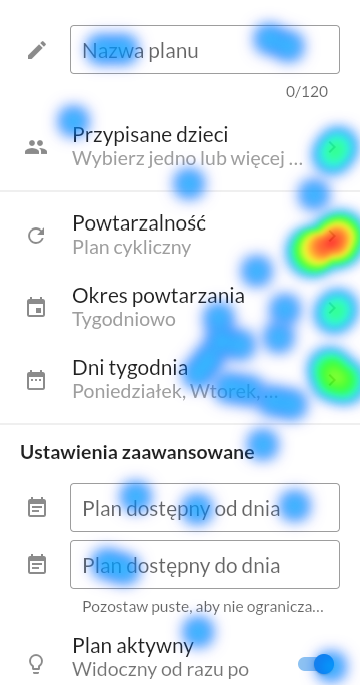
\includegraphics[width=.9\linewidth]{\chapterPath/small-screen.png}
\end{minipage}
\begin{minipage}{.48\textwidth}
	\centering
	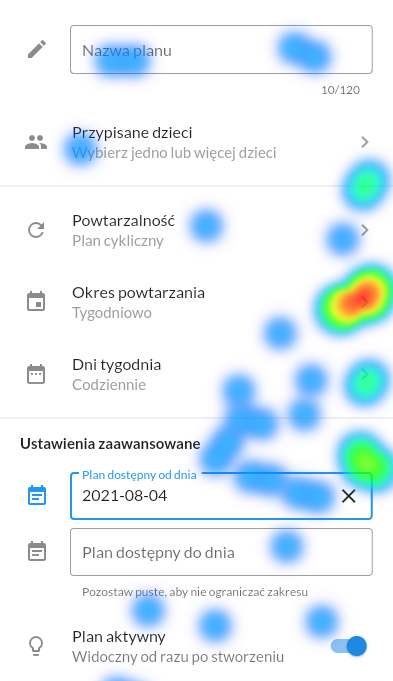
\includegraphics[width=.9\linewidth]{\chapterPath/big-screen.png}
\end{minipage}
\bigskip
\caption{Wpływ różnic~w~wielkościach ekranów}
\label{fig:screen_sizes}
\end{figure}

	\section{Zapewnianie jakości}
Twórcy języka Dart,~w~którym pisane~są~aplikacje~i~narzędzia działające~na~platformie Flutter, opublikowali szereg wytycznych~i~wskazówek mających podnieść jakość, zwięzłość, czytelność~i~niezawodność kodu \cite{Effective_Dart}. Stworzyli też narzędzia pomagające deweloperom~w~trzymaniu się tych wytycznych~i~automatyzacji niektórych powtarzalnych czynności \cite{Dart_SDK}.

\subsection{Używane narzędzia}

\paragraph{Analiza statyczna}
\label{par:static_analysis}
Linter jest kolekcją stale rozwijanych reguł języka Dart określających błędy oraz dobre praktyki konstrukcji~i~stylu kodu \cite{Dart_Lints}. Każdy projekt  może dostosować listę reguł, które zostaną zaaplikowane~do~znajdującego się~w~nim kodu. Narzędzie \codeinline{dart analyze} służy~do~przeprowadzania statycznej analizy kodu, opierając się~o~wybrane reguły \cite{Dart_Analyze}. Wskazuje ono programiście potencjalne błędy~i~problemy~w~kodzie~bez~uruchamiania go. Duży wybór~i~różnorodność reguł (aktualnie jest ich prawie 200) pomaga uniknąć części problemów~i~utrzymać jakość pisanego programu~w~trakcie jego powstawania.

\paragraph{Formatowanie}
\label{par:dart_format}
Narzędzie \codeinline{dart format} zmienia ułożenie znaków białych~w~plikach programu, dostosowując~go~do~wytycznych twórców języka \cite{Dart_Format}. Dzięki określeniu oficjalnego stylu formatowania kodu trzymające się niego projekty pozostają wizualnie spójne, rozwiązując problem niejednolitego formatowania części napisanych~przez~różnych deweloperów.

\subsection{Testy oprogramowania}
Testy jednostkowe~są~podstawową metodą weryfikacji działania poszczególnych komponentów programu komputerowego. Dzięki narzędziu \codeinline{flutter_test} możliwe jest pisanie testów~nie~tylko~dla zaimplementowanej logiki,~ale~także dla komponentów bezpośrednio wchodzących~w~interakcje~z~platformą Flutter. Pozwala ona~na~symulowanie zdarzeń takich jak interakcje użytkownika~i~weryfikację poprawnej reakcji programu. 
 
\paragraph{Pokrycie testami}
\label{par:test_coverage}
Narzędzie Round Spot zostało pokryte testami jednostkowymi weryfikującymi jego poprawne działanie. Do~mierzenia pokrycia testami, czyli części kodu źródłowego programu wykonywanego podczas działania testów, używany jest serwis \href{https://codecov.io/}{codecov.io}. Jedną~z~jego zalet jest wizualizacja pokrycia~w~formie wykresu pierścieniowego,~w~którym kolejne poziomy odpowiadają folderom~w~projekcie, zewnętrzne łuki plikom kodu źródłowego~a~kolory procentowi ich pokrycia testami \cite{RS_Coverage}. Aktualne pokrycie projektu wynosi ponad 50\%. Duża część nieprzetestowanego jeszcze kodu znajduje się~w~menedżerze tła, który sprawia~pod~tym względem trudności, ponieważ operuje~na~binarnych danych obrazów, przetwarzając~i~łącząc je. W~planach~na~przyszłość zawarte jest zwiększenie liczby testów~i~pokrycie nimi całego projektu \ref{sec:future_coverage}.

\bigskip
\img{\chapterPath/coverage_sunburst.png}{Wykres pierścieniowy \ang{sunburst} pokrycia projektu Round Spot testami}{rs_coverage}{.45}

\subsection{Ciągła integracja}
\label{sec:rs_ci}
Praktyka stosowana~w~trakcie rozwoju oprogramowania, polegająca~na~częstym, regularnym włączaniu (integracji) bieżących zmian~w~kodzie~do~głównego repozytorium~i~każdorazowej weryfikacji zmian, poprzez zbudowanie projektu (jeśli jest taka potrzeba) oraz wykonanie testów jednostkowych \cite{CI_definition}.

Repozytorium GitHub używane~do~przechowywania projektu oferuje wbudowaną platformę~do~ciągłej integracji, GitHub Actions, dostępną~za~darmo dla projektów~o~otwartym kodzie źródłowym \cite{RoundSpot_Actions}. Została ona skonfigurowana~tak,~aby przy każdej opublikowanej~w~repozytorium zmianie weryfikować brak problemów zgłaszanych~przez~\hyperref[par:static_analysis]{analizę statyczną}~i~poprawne \hyperref[par:dart_format]{sformatowanie} kodu. Uruchamia też testy jednostkowe, weryfikując poprawne działanie poszczególnych komponentów,~po~czym aktualizuje informacje zawarte~na~portalu \href{https://codecov.io/}{codecov.io} \cite{RS_Coverage} nowymi danymi dotyczącymi pokrycia testami. Jeśli którakolwiek~z~wykonywanych czynności~nie~powiedzie się (wykryte zostaną problemy, kod jest niepoprawnie sformatowany~lub~testy kończą się niepowodzeniem), akcja kończy się niepowodzeniem,~a~informacja~o~tym jest wyświetlana~na~stronie głównej repozytorium.

	\section{Przygotowanie~do~wydania}

\subsection{Dokumentacja}
Każdy opublikowany pakiet powinien posiadać dokumentację ułatwiającą jego użycie. Twórcy języka Dart udostępnili wytyczne standaryzujące sposób pisania dokumentacji~w~plikach źródłowych \cite{Dart_Doc_Guidelines}. Komentarze zaczynające się~od~potrójnego znaku \codeinline{///} zawierają opisy elementów~i~struktur, które poprzedzają. Istnieje też możliwość formatowania ich zawartości (np. \codeinline{_kursywa_}), odwoływania się~do~innych fragmentów kodu (\codeinline{[Klasa.pole]}) oraz zamieszczania przykładów (\codeinline{`kod`} oraz \codeinline{```wielolinijkowy fragment kodu```}).

\bigskip
\begin{lstlisting}[language=dartcomment,caption={Fragment dokumentacji zawartej~w~kodzie źródłowym pakietu},label=lst:rs_docs]
/// Initializes the _Round Spot_ library.
///
/// Takes a [child] widget, an optional [config],
/// a [loggingLevel] which defaults to [LogLevel.off]
/// and output callbacks ([localRenderCallback] and [dataCallback]) 
/// that must be set depending on the [Config.outputType] requested.
///
/// Should be invoked in `main()` or otherwise wrap the [MaterialApp] widget:
/// ```dart
/// void main() {
///   runApp(initialize(
///     child: Application()
///   ));
/// }
/// ```
\end{lstlisting} 


Aby umożliwić korzystanie~z~dokumentacji~w~wygodnej~i~interaktywnej formie stworzone zostało narzędzie \codeinline{dartdoc} \cite{Dart_Doc} przetwarzające komentarze~z~plików kodu źródłowego projektu~do~postaci strony internetowej. Przetwarzana treść jest formatowana,~a~w~miejsce odwołań~są~wstawiane linki. Wynik przetwarzania listingu \ref{lst:rs_docs} znajduje się~na~rysunku \ref{fig:rs_html_docs}. Powtarzające się fragmenty mogą zostać wstawione~w~szablony, których treść zostanie skopiowana~we~wskazane miejsca podczas przetwarzania. Podczas publikacji pakietu~w~repozytorium \href{https://pub.dev/}{pub.dev} strony~z~dokumentacją~są~automatycznie tworzone~i~umieszczane~w~serwisie, zapewniając łatwy dostęp każdemu, kto chce użyć pakietu \cite{RS_Documentation}.

\bigskip
\img{\chapterPath/rs_docs.png}{Fragment przetworzonej~na~stronę internetową dokumentacji}{rs_html_docs}{.8}

\subsection{Przykład}
\label{sec:rs_example}
Sugeruje się, żeby każdy opublikowany pakiet posiadał dołączony przykład ilustrujący sugerowany sposób jego użycia. Powinien być jak najprostszy, przy czym jednocześnie wyraźnie pokazywać funkcjonalność oferowaną~przez~zawierający~go~pakiet. W~tym przypadku przykład zawiera prostą aplikację~z~dwoma ekranami~i~przewijaną listą wraz z instrukcją jak uruchomić kod~i~uzyskać pliki map cieplnych używając lokalnego przetwarzania danych \cite{RS_Example}.

\subsection{Repozytorium kodu}
Kod źródłowy projektu jest publicznie dostępny~w~serwisie GitHub \cite{RoundSpot_GitHub}. Serwis został wybrany~z~powodu popularności~i~liczby oferowanych funkcji. Akcje umożliwiają stworzenie procesu \hyperref[sec:rs_ci]{ciągłej integracji} opartego~o~konteneryzację. Zakładka problemów \ang{Issues} pozwala każdemu~na~zadawanie pytań~i~zgłaszanie uwag podczas gdy projekty oferują prostą tablicę typu Kanban ułatwiającą organizację zadań. Na~stronie głównej projektu wyświetlany jest plik informacyjny \codeinline{README.md} zawierający podstawowe informacje~i~pierwsze kroki. Kod udostępniony jest~na~otwartej licencji MIT.

\subsection{Pub.dev}
Oficjalne repozytorium otwartych~i~darmowych pakietów stworzonych~w~języku Dart oraz~na~platformie Flutter. Na~głównej stronie pakietu (rysunek \ref{fig:rs_pub_dev}) wyświetlony jest jego plik \codeinline{README.md}. Pozostałe zakładki zawierają między innymi historię zmian (braną~z~pliku \codeinline{CHANGELOG.md}), dodany \hyperref[sec:rs_example]{przykład} oraz instrukcje instalacji. Po~prawej stronie znajduje się kolumna zawierająca dodatkowe informacje~i~linki~do~repozytorium, dokumentacji~i~licencji \cite{RS_Pub_dev}.

\paragraph{Ocena} Każdy pakiet jest automatycznie oceniany~w~skali 0-130. Na~ocenę wpływ~ma~między innymi wynik działania \hyperref[par:static_analysis]{analizy statycznej}, obecność dokumentacji, wsparcie dostępnych platform oraz najnowszych funkcji języka.

\bigskip
\img{\chapterPath/rs_pub_dev.png}{Strona główna pakietu~w~repozytorium pub.dev}{rs_pub_dev}{1}



\end{chapter}

\begin{chapter}{Ewaluacja narzędzia}
	\newcommand{\chapterPath}{chapters/RS_Evaluation}

	\section{Przygotowanie}
Do przeprowadzenia testów oraz ewaluacji potrzebna była odpowiednia aplikacja zbudowana na platformie Flutter. Wymaganiem był swobodny dostęp do jej kodu źródłowego, możliwość jego modyfikacji oraz ponownego zbudowania. Aplikacja powinna być umiarkowanie rozbudowana, z minimum ośmioma ekranami, przestrzeniami przewijanymi oraz elementami nawigacji. Podczas jej używania powinien być wymagany dostęp do internetu aby zapewnić możliwość zapisu zebranych danych. 

\subsection{Fokus}
Aplikacja mobilna Fokus została stworzona w ciągu ostatniego roku w ramach projektu grupowego przez zespół prowadzony przez autora tej pracy. Jej celem jest pomaganie dzieciom w wykonywaniu codziennych zadań pod kontrolą opiekuna. Tworzy on plany i zadania do zrobienia za które dziecko dostaje punkty wydawane na dodane przez opiekuna nagrody. Aplikacja dobrze nadaje się do wykorzystania do przeprowadzenia na niej ewaluacji. Jest wystarczająco rozbudowana, dzieląc się na sekcje dostępne dla opiekuna i dziecka, z których każda zawiera około osiem ekranów. Zawiera różnorodne elementy interfejsu użytkownika, takie jak przewijane karty, zakładki, wyskakujące okna, paski nawigacji oraz pola do wprowadzania danych. Jest też aktywnie testowana przez grupę użytkowników.

\subsection{Integracja}
Proces integracji narzędzia w aplikacji Fokus składał się z konfiguracji oraz instrumentacji interfejsu użytkownika. Detektory interakcji zostały umieszczone na około każdego obszaru przewijanego oraz tych wyskakujących okien które na to pozwalały. Do konfiguracji posłużyły dwie z usług oferowanych w ramach używanej przez aplikację platformy \nameref{sec:firebase}. Moduł zdalnej konfiguracji (Remote Config) jest odpowiedzialny za pobieranie aktualnie ustawionej w formie pliku json \hyperref[sec:rs_config]{konfiguracji}. Dzięki temu parametry działania związane ze specyfiką zbierania danych do map cieplnych mogą zostać zmienione w dowolnym momencie bez instalacji nowej wersji aplikacji przez testerów. Po zakończeniu ewaluacji kolekcja danych może też zostać zdalnie wyłączona. Firebase oferuje też usługę dysku w chmurze (Firebase Storage) która została użyta w celu zebrania danych ze wszystkich urządzeń użytkowników biorących udział w ewaluacji. Z tej centralnej lokalizacji pliki mogą zostać łatwo pobrane i przetworzone na mapy cieplne.

	\section{Weryfikacja}
Weryfikacja działania została przeprowadzona~przez~autora pracy~na~gotowej~do~ewaluacji wersji aplikacji. Jej celem było potwierdzenie poprawności działania mechanizmu zbierania danych oraz wyciągnięcie pierwszych wniosków~o~przydatności~i~działaniu narzędzia.

\subsection{Wskazanie popularności elementów}
Przegląd map cieplnych pozwala~na~łatwą identyfikację częściej~i~rzadziej używanych funkcji, ekranów~i~elementów interfejsu aplikacji. Szczególnie dobrze nadają się~do~tego celu mapy kumulacyjne elementów nawigacji. Testowana aplikacja posiada dolny pasek nawigacji dzielący~ją~na~trzy obszary: panel, plany oraz nagrody. Na mapie \ref{fig:rs_bottom_nav_bar} można zauważyć,~że~pierwsza zakładka jest używana najczęściej podczas gdy pozostałe dwie~są~wybierane~przez~użytkowników~w~przybliżeniu~tak~samo często.

\bigskip
\img{\chapterPath/[bottom-nav-bar].png}{Pasek nawigacji testowanej aplikacji}{rs_bottom_nav_bar}{.7}

\subsection{Ekrany~i~obszary przewijane}
Ekrany posiadające potencjalnie przewijane obszary muszą być rozdzielone~na~mapę interakcji~ze~statycznymi elementami interfejsu oraz mapę zawartości znajdującej się~w~przewijanym polu. Na~obrazkach \ref{fig:rs_panel_parts} przedstawiony jest przykład takiej sytuacji. Po~prawej stronie znajduje się mapa obszaru przewiniętego~przez~użytkownika. Można też wywnioskować,~że~większość~z~zarejestrowanych dotknięć ekranu znajdujących się~w~pionowej osi centralnej ekranu była spowodowana jego przewijaniem. 

\bigskip
\begin{figure}[H]
\centering
\begin{minipage}{.35\textwidth}
	\centering
	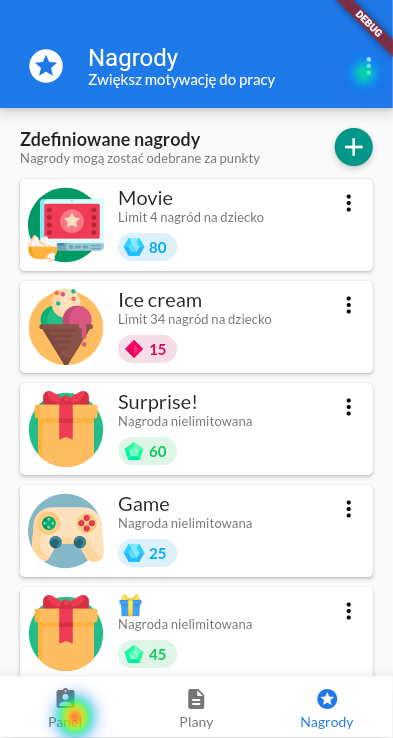
\includegraphics[width=.9\linewidth]{\chapterPath/caregiver-awards-page.png}
\end{minipage}
\begin{minipage}{.3\textwidth}
	\centering
	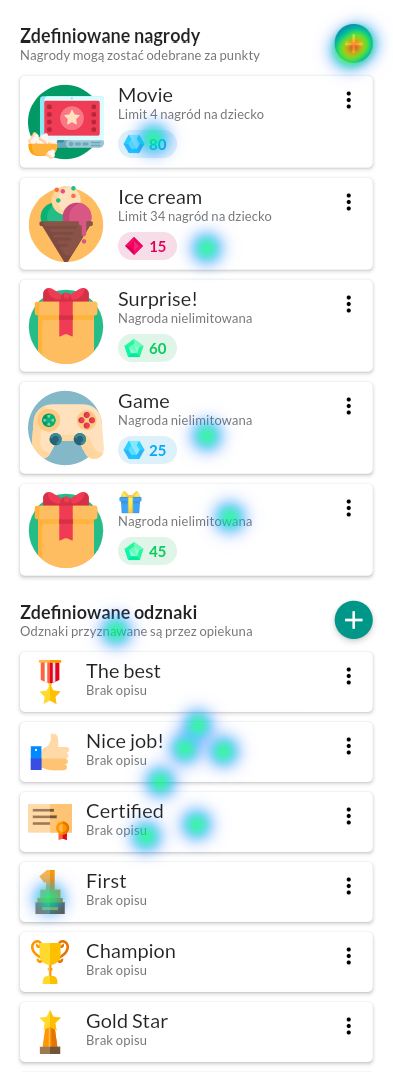
\includegraphics[width=.9\linewidth]{\chapterPath/[main-scroll-area] caregiver-awards-page.png}
\end{minipage}
\bigskip
\caption{Ekran nagród użytkownika}
\label{fig:rs_panel_parts}
\end{figure}

\subsection{Niewidoczne elementy}
Aktualnie~w~niektórych przypadkach,~na~przykład kiedy~w~aplikacji używany jest gotowy komponent, niemożliwe może być zawarcie~go~na~mapie cieplnej. Taki przypadek przedstawiony jest na rysunku \ref{fig:rs_reward_form}. Pomimo~że~w~aplikacji użytkownik wybiera ikonę nagrody~z~wysuwającej się~od~dołu karty,~na~mapie cieplnej karta~nie~jest widoczna, mogąc powodować mylne zakwalifikowanie interakcji jako dotknięcia pustej przestrzeni~na~ekranie. To~aktualne ograniczenie zostało opisane jako jeden~z~punktów~w~sekcji \nameref{sec:future_work}.

\bigskip
\begin{figure}[H]
\centering
\begin{minipage}{.3\textwidth}
	\centering
	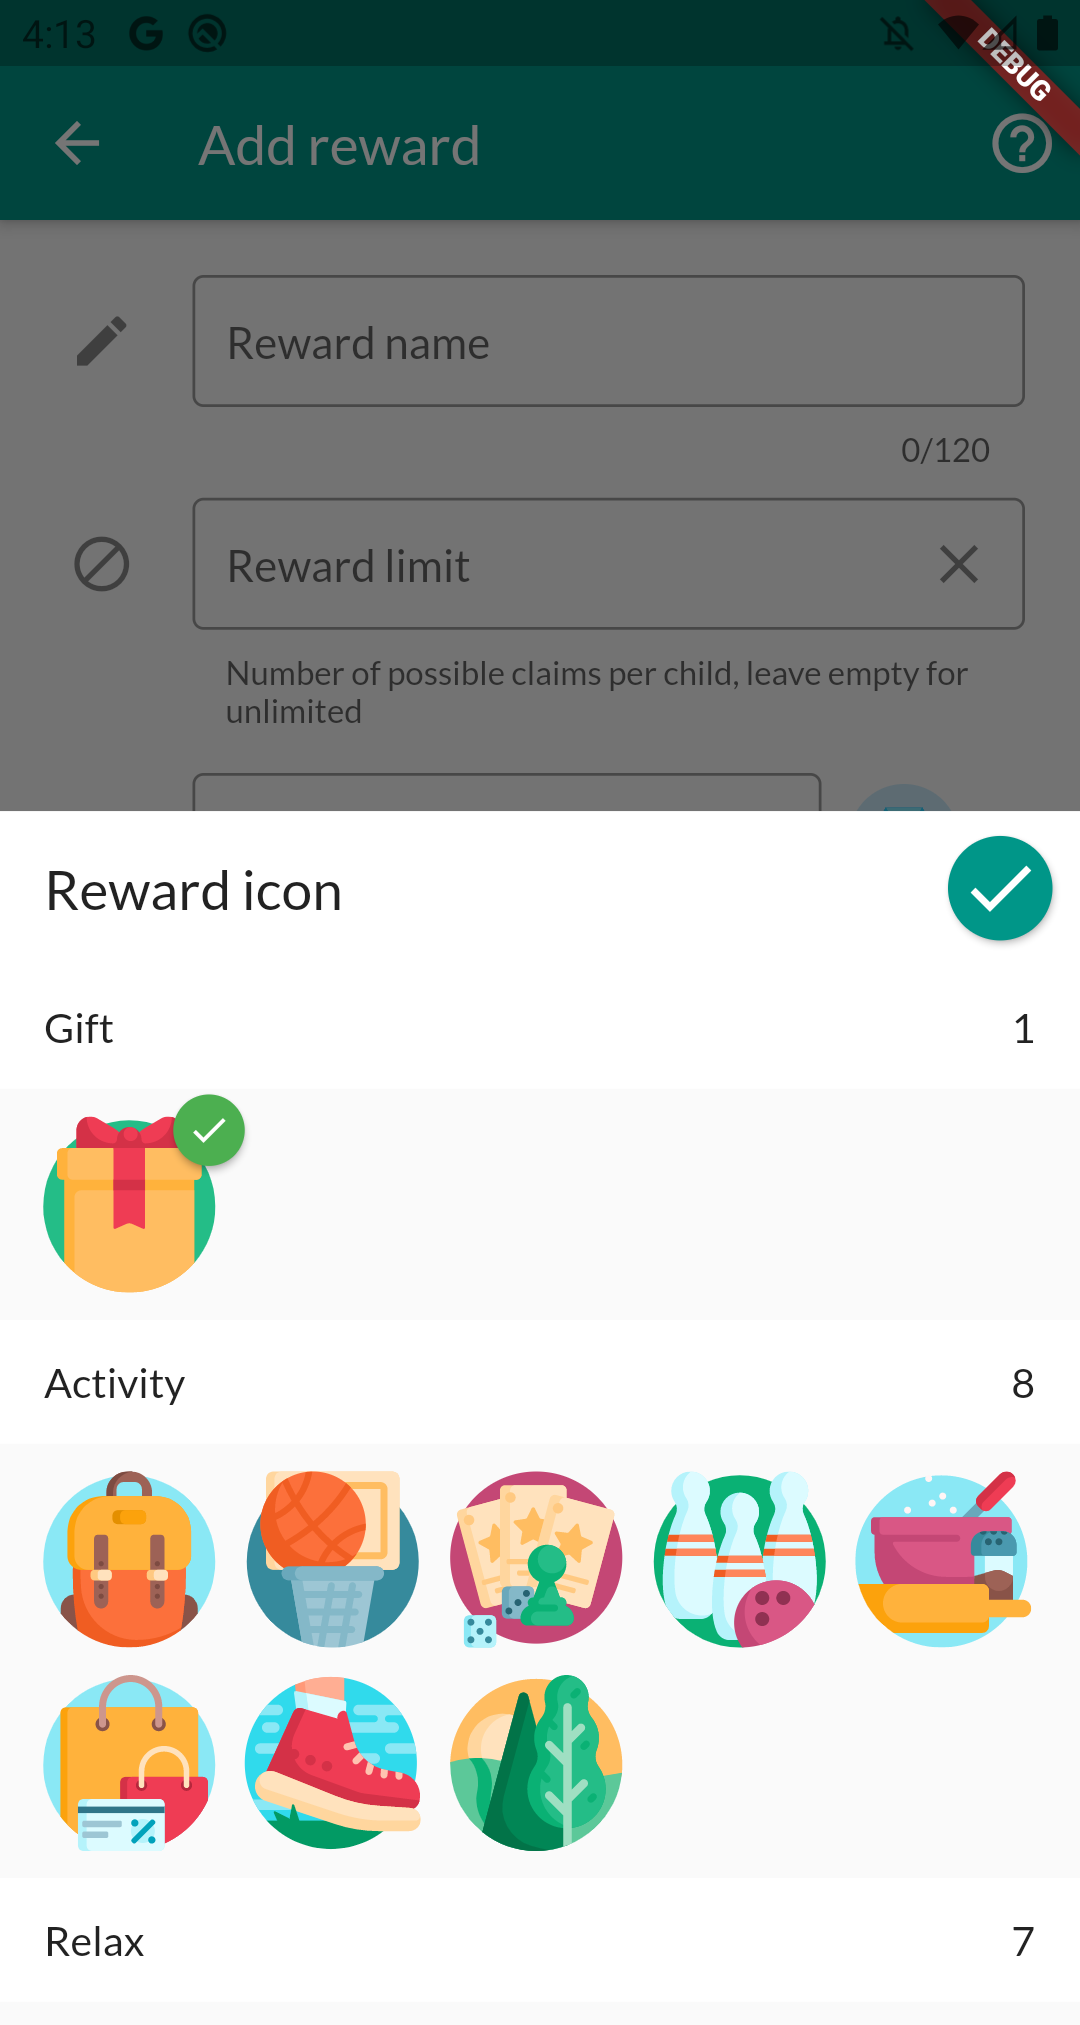
\includegraphics[width=.9\linewidth]{\chapterPath/smart-select-popup.png}
\end{minipage}
\begin{minipage}{.3\textwidth}
	\centering
	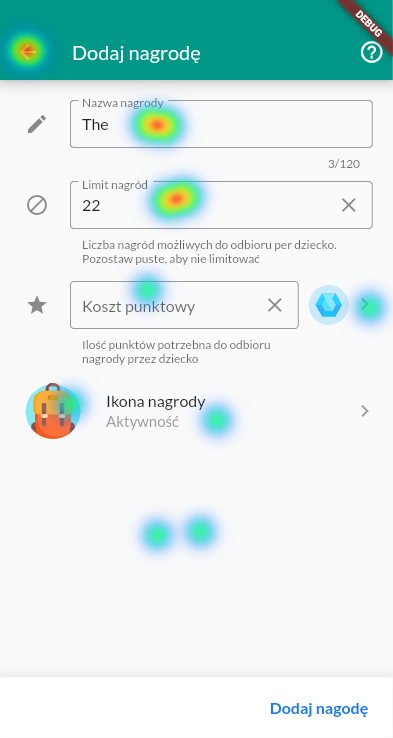
\includegraphics[width=.9\linewidth]{\chapterPath/caregiver-rewards-form-page.png}
\end{minipage}
\bigskip
\caption{Ekran tworzenia nagrody~i~powstała mapa cieplna}
\label{fig:rs_reward_form}
\end{figure}

\subsection{Zmienne elementy}
W przypadku przewijanych obszarów zawierających animowane (zmieniające zawartość, wielkość~lub~kształt) elementy, tło stworzonych map może~nie~być spójne. Wynika~to~z~opisanego już mechanizmu stopniowego tworzenia tła~z~części wyświetlanych~na~ekranie~w~danym momencie. W przykładzie \ref{fig:rs_rating_cards}~po~lewej stronie widać widok kart~na~ekranie aplikacji. W~trakcie przewijania widok jest animowany, powodując powiększenie aktualnie wyświetlanej~na~środku karty. Po~prawej stronie umieszczona została mapa cieplna złożona~z~trzech kart~po~ich przewinięciu~przez~użytkownika. Z~powodu połączenia obrazków,~na~których~ta~sama karta~ma~różną wielkość, obie boczne karty zawierają defekty graficzne. Pomimo tego ograniczenia wynikowe tło mapy cieplnej nadal spełnia swoją funkcję, pozwalając~na~umiejscowienie interakcji użytkowników~na~ekranie.

\bigskip
\begin{figure}[H]
\begin{minipage}{.25\textwidth}
	\centering
	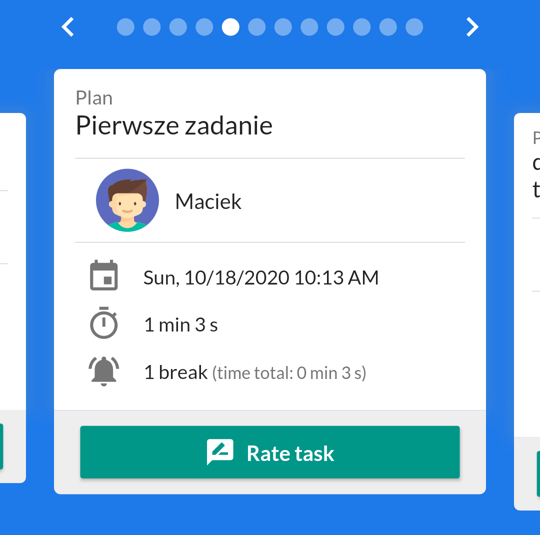
\includegraphics[width=.9\linewidth]{\chapterPath/rating_cards-app.png}
\end{minipage}
\begin{minipage}{.74\textwidth}
	\centering
	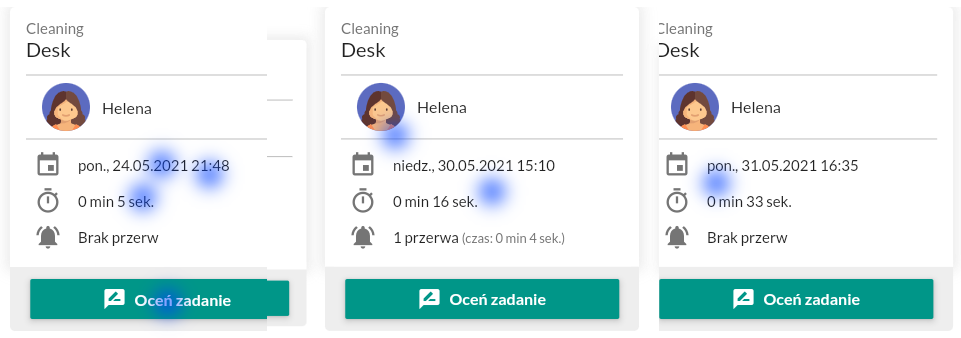
\includegraphics[width=.9\linewidth]{\chapterPath/[rating-cards]-caregiver-rating-page.png}
\end{minipage}
\bigskip
\caption{Widok kart~w~aplikacji oraz~na~mapie cieplnej}
\label{fig:rs_rating_cards}
\end{figure}

	\section{Ewaluacja}

\subsection{Fokus}
przygotowanie, integracja 

\subsection{Korzyści}
Narzędzie pozwala na automatyczne zbieranie cennych danych których pozyskanie w innym przypadku wymagałyby zorganizowania czasochłonnych testów. Dzięki intuicyjnej, graficznej reprezentacji interakcji połączonej z dobrą znajomością interfejsu jego twórca jest w stanie znacznie szybciej diagnozować problemy które mają użytkownicy w trakcie używania aplikacji. Nagrania zebrane ze zwykle przeprowadzanych testów są zazwyczaj cięższe i wolniejsze w analizie z powodu konieczności manualnego spisywania wydarzeń, braku informacji o dokładnych miejscach interakcji oraz częściowym zasłanianiu ekranu przez rękę użytkownika. 

	\section{Dalszy rozwój}
\subsection{Typy interakcji}
Mysz, gesty, drag

\subsection{Platformy}
Web, Win, Mac, Lin 

\subsection{Zawartość}
Dynamic content

\subsection{Automatyczna instrumentacja}

\subsection{Prywatność}
Blur

\subsection{Przetwarzanie lokalne}
serwer, mapy całego ruchu bez podziału na urządzenia


\end{chapter}

 \begin{chapter}{Podsumowanie}
	\newcommand{\chapterPath}{chapters/Summary}

	Pierwszym celem pracy była analiza i porównanie z sobą różnych mechanizmów monitorowania użytkowników, głównie w kontekście aplikacji mobilnych. Drugie wskazane w temacie pracy do realizacji zadanie dotyczyło wybrania jednego z analizowanych mechanizmów i zaimplementowania go w istniejącej aplikacji terapeutycznej. 
	
	\section{Osiągnięte rezultaty}
	
	\subsection{Przegląd mechanizmów}
	Wykonana analiza istniejących mechanizmów monitorujących zajmująca rozdziały \ref{cha:existing_solutions} do \ref{cha:heat_maps} rozpatruje temat z możliwie wielu perspektyw. Opisane zostały przykłady gotowych rozwiązań, takich jak aplikacje, mechanizmy systemów mobilnych i komercyjne platformy \ang{frameworks} oferujące usługi z zakresu monitorowania. Wykonany systematyczny przegląd literatury naukowej skupia się za to na aspekcie wykorzystania czujników w urządzeniach takich jak smartfony w celu wykrywania i opisu aktywności ludzkich. Przedstawione zostały także przykłady popularnych produktów z wybranego do implementacji w dalszej części pracy typu rozwiązań tworzących mapy cieplne interakcji użytkowników. Wymienione w każdej kategorii przykłady są ze sobą porównane pod względem funkcji, podobieństw i zaawansowania.
	
	\subsection{Autorskie rozwiązanie}
	Wybrany do implementacji aspekt monitorowania polega na obserwacji interakcji użytkowników z interfejsem aplikacji i ich późniejszym przetwarzaniu do graficznej formy map cieplnych poszczególnych ekranów. Zamiast bezpośredniej implementacji w docelowej aplikacji terapeutycznej powstało uniwersalne narzędzie które może zostać wykorzystane w dowolnej aplikacji opartej o platformę Flutter, co znacznie zwiększa jego potencjalny obszar wpływu. Praca nad tworzeniem rozwiązania była przeprowadzona według najlepszych standardów jakości kodu oraz jego testowania. Wykonana ewaluacja składająca się ze wstępnej weryfikacji oraz walidacji z udziałem testerów wykazała słabe i mocne strony działania narzędzia potwierdzając jednocześnie jego przydatność w analizie dostępności interfejsu i zachowań użytkowników.
	
	\section{Napotkane wyzwania}
	Podczas procesu implementacji i ewaluacji tworzonego narzędzia wystąpiło wiele problemów stanowiących poważne wyzwania stojące na drodze do poprawnie działającego, użytecznego rozwiązania. Część z nich wynikała z potrzeby uzyskania bardzo specyficznie określonego zestawu danych który częściowo wychodził poza założenia na których zbudowany został interfejs programistyczny \ang{Application Programming Interface - API} platformy Flutter. Wyzwaniami okazały się też właściwa architektura i przepływ przetwarzania danych dający odpowiednią swobodę, a także rysowanie samej mapy cieplnej w atrakcyjny wizualnie i przejrzysty w analizie sposób.
	
	\section{Sformułowane wnioski}
	
	\subsection{Literatura naukowa}
	płytka, powtarzalna (wybrany zbiór - reprezentatywny?), z~wyjątkami
	
	\subsection{Narzędzie monitorujące}
	duże aspektów do~wzięcia pod~uwagę, miejsca na~rozwój, działająca podstawa wnosząca wartość przy badaniach
	
\end{chapter}



\cleardoublepage
\phantomsection
\bibliographystyle{unsrt}
\renewcommand\bibname{Wykaz literatury}
\bibliography{bibtex/SLR,bibtex/existing_docs,bibtex/heat_map}
\addcontentsline{toc}{chapter}{WYKAZ LITERATURY}

\cleardoublepage
\phantomsection
\addcontentsline{toc}{chapter}{\listtablename}
\listoftables
\renewcommand{\baselinestretch}{1.3}\normalsize

\cleardoublepage
\phantomsection
\renewcommand{\baselinestretch}{1.0}\normalsize
\addcontentsline{toc}{chapter}{\listfigurename}
\listoffigures


\cleardoublepage
\phantomsection
\renewcommand\lstlistlistingname{Spis listingów}
\addcontentsline{toc}{chapter}{\lstlistlistingname}
\lstlistoflistings

\annex{Wymagania narzędzia monitorującego}{tool_requirements}

\section*{Wymagania funkcjonalne}
\newcommand\tabreq[3]{\ref{req:#1} & #2 & #3 \\\midrule}
\newcommand\reqheader[2]{\item \label{req:#1} {\it #2}:}

Poniżej znajduje się spis zidentyfikowanych dla tworzonego narzędzia wymagań funkcjonalnych. Priorytety zostały wyrażone~w~następującej skali: {\bf 3} - {\it największy}~do~{\bf 1} - {\it najmniejszy}.

\centertable{\toprule
	\textbf{ID} & \textbf{Nazwa} & \textbf{Priorytet} \\\toprule 
	\tabreq{screen_touch}{Rejestrowanie dotknięć ekranu}{3}
	\tabreq{heat_map}{Tworzenie map cieplnych}{3}
	\tabreq{per_screen}{Podział danych~na~ekrany aplikacji}{3}
	\tabreq{time_periods}{Podział danych~na~okresy czasowe}{3}
	\tabreq{scrolling}{Wsparcie dla przewijanej treści}{3}
	\tabreq{numer_data}{Eksport nieprzetworzonych danych}{2}
	\tabreq{session_config}{Konfiguracja parametrów zbieranych danych}{2}
	\tabreq{store_config}{Wybór sposobu składowania danych}{2}
	\tabreq{event_grouping}{Grupowanie interakcji~ze~względu~na~współrzędne}{2}
	\tabreq{screen_selection}{Wybór nagrywanych ekranów aplikacji}{1}
	\tabreq{on_off}{Możliwość wyłączenia działania narzędzia}{1}
	\tabreq{dynamic_config}{Opcja zmiany konfiguracji~w~trakcie działania}{1}
	\tabreq{ui_size}{Możliwość dostosowania rozmiaru interfejsu}{1}
}{l l r}{Wykaz wymagań funkcjonalnych narzędzia}{tool_requirements}

\begin{enumerate}[label=\textbf{F.\arabic*}]
	\reqheader{screen_touch}{Rejestrowanie dotknięć ekranu} Jako podstawowa forma interakcji~z~urządzeniem mobilnym dotknięcia ekranu stanowią główne źródło danych~do~przetwarzania~przez~narzędzie.
	\reqheader{heat_map}{Tworzenie map cieplnych} Podstawowym celem narzędzia jest przetwarzanie interakcji użytkownika~z~aplikacją~na~ich graficzną reprezentację~w~formie mapy cieplnej. 
	\reqheader{per_screen}{Podział danych~na~ekrany aplikacji} Interakcje dotyczą konkretnego elementu interfejsu. Zbierane dane muszą być przetwarzane~w~kontekście ekranu aplikacji, którego dotyczą. Mapy cieplne \ref{req:heat_map} powinny być nałożona~na~zdjęcie odpowiedniego ekranu~w~celu łatwej identyfikacji elementów interfejsu,~z~którymi zachodzi interakcja.
	\reqheader{time_periods}{Podział danych~na~okresy czasowe} Dane zbierane~w~ramach każdego ekranu muszą zostać podzielone~na~rozsądne grupy,~na~podstawie których będą tworzone pojedyncze mapy cieplne. Podział ten powinien jednocześnie~nie~być zbyt drobny, aby zapewnić optymalną liczbę punktów~do~przetwarzania, oraz~w~miarę możliwości zgadzać się~z~sesjami użycia aplikacji rozdzielonymi okresami bezczynności.
	\reqheader{scrolling}{Wsparcie dla przewijanej treści} Narzędzie powinno identyfikować obszary interfejsu, które mogą być przewijane~i~brać~je~pod~uwagę przy przetwarzaniu danych. W~przeciwnym przypadku interakcje dotyczące przewijanych elementów będą wizualizowane~w~nieprawidłowych miejscach.
	\reqheader{numer_data}{Eksport nieprzetworzonych danych} Oprócz reprezentacji graficznej narzędzie powinno oferować możliwość zapisywania surowych danych~o~współrzędnych~i~czasie pojedynczych interakcji. Pozwoli~to~na~ich swobodne przetworzenie według potrzeby twórcy aplikacji używającego narzędzia.
	\reqheader{session_config}{Konfiguracja parametrów zbieranych danych} Parametry umożliwiające skonfigurowanie procesu zbierania danych takie jak minimalna ilość wykonanych dotknięć ekranu oraz maksymalna długość bezczynności przed zakończeniem rejestrowania interakcji.
	\reqheader{store_config}{Wybór sposobu składowania danych} Aby dane zbierane~przez~narzędzie mogły być przeanalizowane, muszą zostać wysłane~i~zapisane. Narzędzie musi oferować mechanizm przekazywania przetworzonych~przez~siebie danych~w~celu ich zapisania.
	\reqheader{event_grouping}{Grupowanie interakcji~ze~względu~na~współrzędne} Blisko położone siebie dotknięcia ekranu najczęściej dotyczą tej samej akcji. Narzędzie powinno grupować takie interakcje, zaznaczając ich intensywność, aby niepotrzebnie~nie~zaszumiać przekazu graficznego.
	\reqheader{screen_selection}{Wybór nagrywanych ekranów aplikacji} Możliwość selekcji podzbioru ekranów,~na~których interakcje będą rejestrowane~i~przetwarzane~w~celu ograniczenia ilości generowanych danych przy rozbudowanych aplikacjach.
	\reqheader{on_off}{Możliwość wyłączenia działania narzędzia} Użytkownicy końcowi zawsze powinni mieć wybór~czy~chcą uczestniczyć~w~zbieraniu jakichkolwiek danych. Dodatkowo pojawia się potrzeba ręcznej kontroli~nad~pracę narzędzia~w~przypadku przeprowadzania zorganizowanych testów. Narzędzie musi zatem oferować możliwość łatwego włączenia~i~wyłączenia.
	\reqheader{dynamic_config}{Opcja zmiany konfiguracji~w~trakcie działania} W~środowisku produkcyjnym aplikacje często działają~w~tle~przez~długi czas. Z~tego powodu ważne jest zapewnienie możliwości zmiany konfiguracji podczas działania aplikacji.
	\reqheader{ui_size}{Możliwość dostosowania rozmiaru interfejsu} Zależnie~od~używanej~przez~aplikację wielkości elementów interfejsu rozmiar tworzonej mapy cieplnej \ref{req:heat_map} oraz grupowany obszar interakcji \ref{req:event_grouping} powinno dać się dostosować. 
\end{enumerate}


\end{document}
